\subsection[\englishfont 2.2 面向车载信息物理融合的通信与计算资源协同优化]{2.2 面向车载信息物理融合的通信与计算资源协同优化}

\begin{frame}{研究贡献}
\newBackground
\begin{center}
\begin{textblock*}{\textwidth}(-2cm,1.8cm)
  \small \englishfont \colorbox{cqublue}{\color{white}{先进的任务调度与资源分配策略是{\color{yellow}{进}}}}
\end{textblock*}
\end{center}

\begin{center}
\begin{textblock*}{\textwidth}(-2cm,2.3cm)
  \small \englishfont \colorbox{cqublue}{\color{white}{{\color{yellow}{一步优化}}\hspace{0.2em}VCPS服务质量的{\color{yellow}{技术支撑}}}}
\end{textblock*}
\end{center}

\begin{center}
\begin{textblock*}{\textwidth}(-1.5cm,3.16cm)
\begin{minipage}[t]{0.75\textwidth}
\begin{itemize}[itemsep=0.2\baselineskip]  \englishfont
	\item[\ding{111}] {{\color{cqublue}{\textbf{问题}}}:协同资源优化 ({\color{red}{CRO}}})
	\item[\ding{111}]  {{\color{cqublue}{\textbf{算法}}}:基于博弈理论的多智能体深度强化学习 ({\color{red}{MAGT}})}
	\begin{itemize}[itemsep=0.2\baselineskip] 
	\begin{small}
		\item[\ding{226}] 问题分解
		\item[\ding{226}] 边缘节点智能体决策任务调度
		\item[\ding{226}] 凸优化最优资源分配
	\end{small}
	\end{itemize}
	\item [\ding{111}]  {{\color{cqublue}{\textbf{实验}}}:有效提高任务完成率}
	\end{itemize}
\end{minipage}
\end{textblock*}
\end{center}

\begin{center}
\begin{textblock*}{\textwidth}(-1.2cm,6.6cm)
\fbox{\begin{minipage}[t]{0.75\textwidth}\englishfont \tiny [3] \underline{\textcolor{cqublue}{XU X}}, LIU K, DAI P, et al. \textcolor{cqublue}{Joint task offloading and resource optimization in NOMA-based vehicular edge computing: A game-theoretic DRL approach}[J]. Journal of Systems Architecture (\textcolor{red}{JSA}), 2023, 134: 102780. 影响因子: 5.836(2021), 4.497(5年)  (中科院SCI 2区)
\end{minipage}}
\fbox{\begin{minipage}[t]{0.75\textwidth}\englishfont \tiny [4] \underline{\textcolor{cqublue}{许新操}}, 刘凯, 刘春晖, 等. \textcolor{cqublue}{基于势博弈的车载边缘计算信道分配方法}[J]. 电子学报, 2021. (CCF T1类中文期刊)
\end{minipage}}
\end{textblock*}
\end{center}

\begin{center}
\begin{textblock*}{\textwidth}(6.5cm,1.6cm)
\begin{figure}
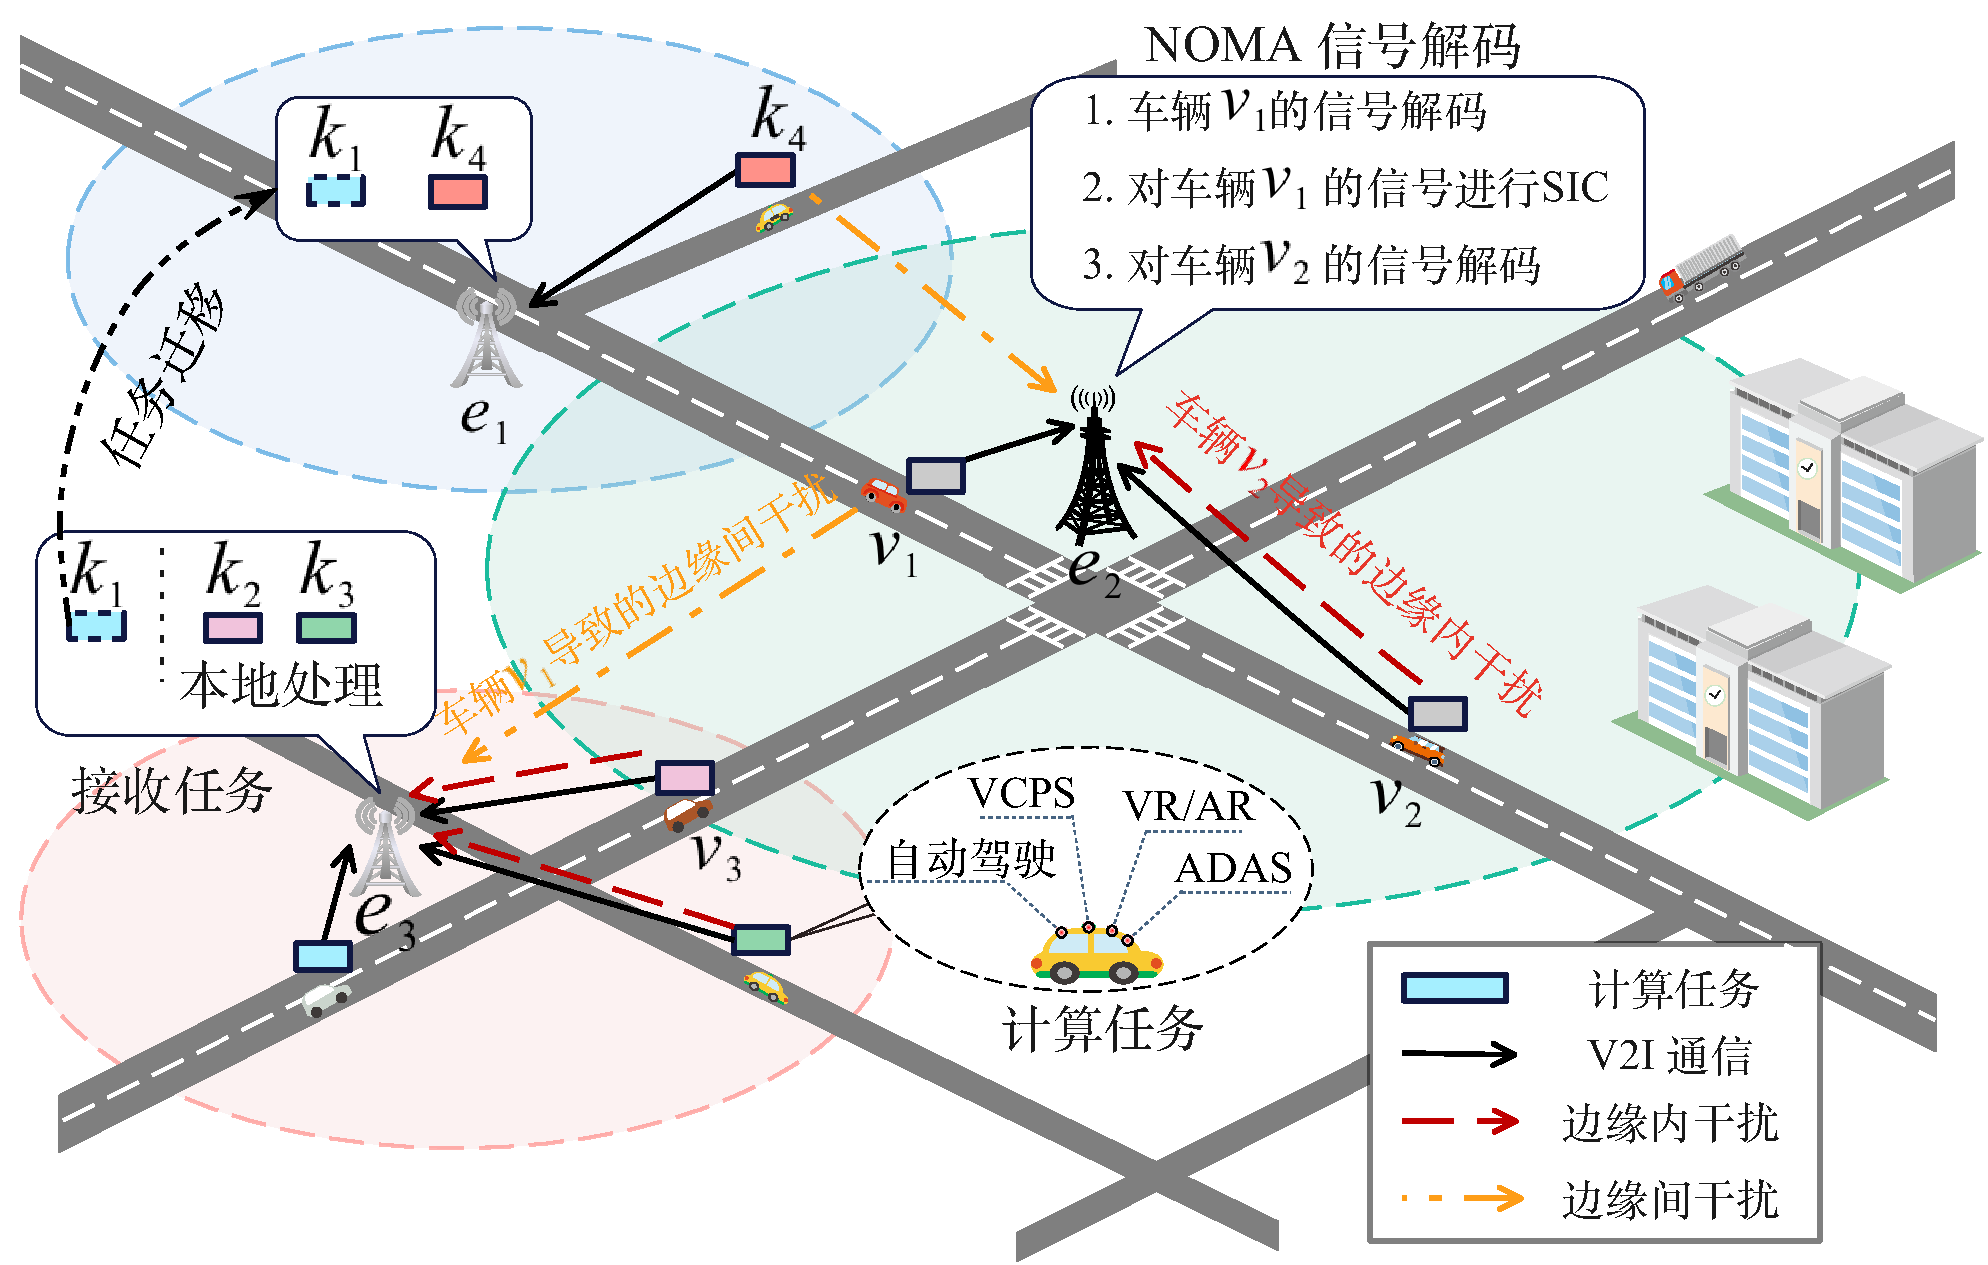
\includegraphics[width=0.3\textwidth]{fig/Fig3-1-noma-architecture.pdf}
\end{figure}
\begin{figure}
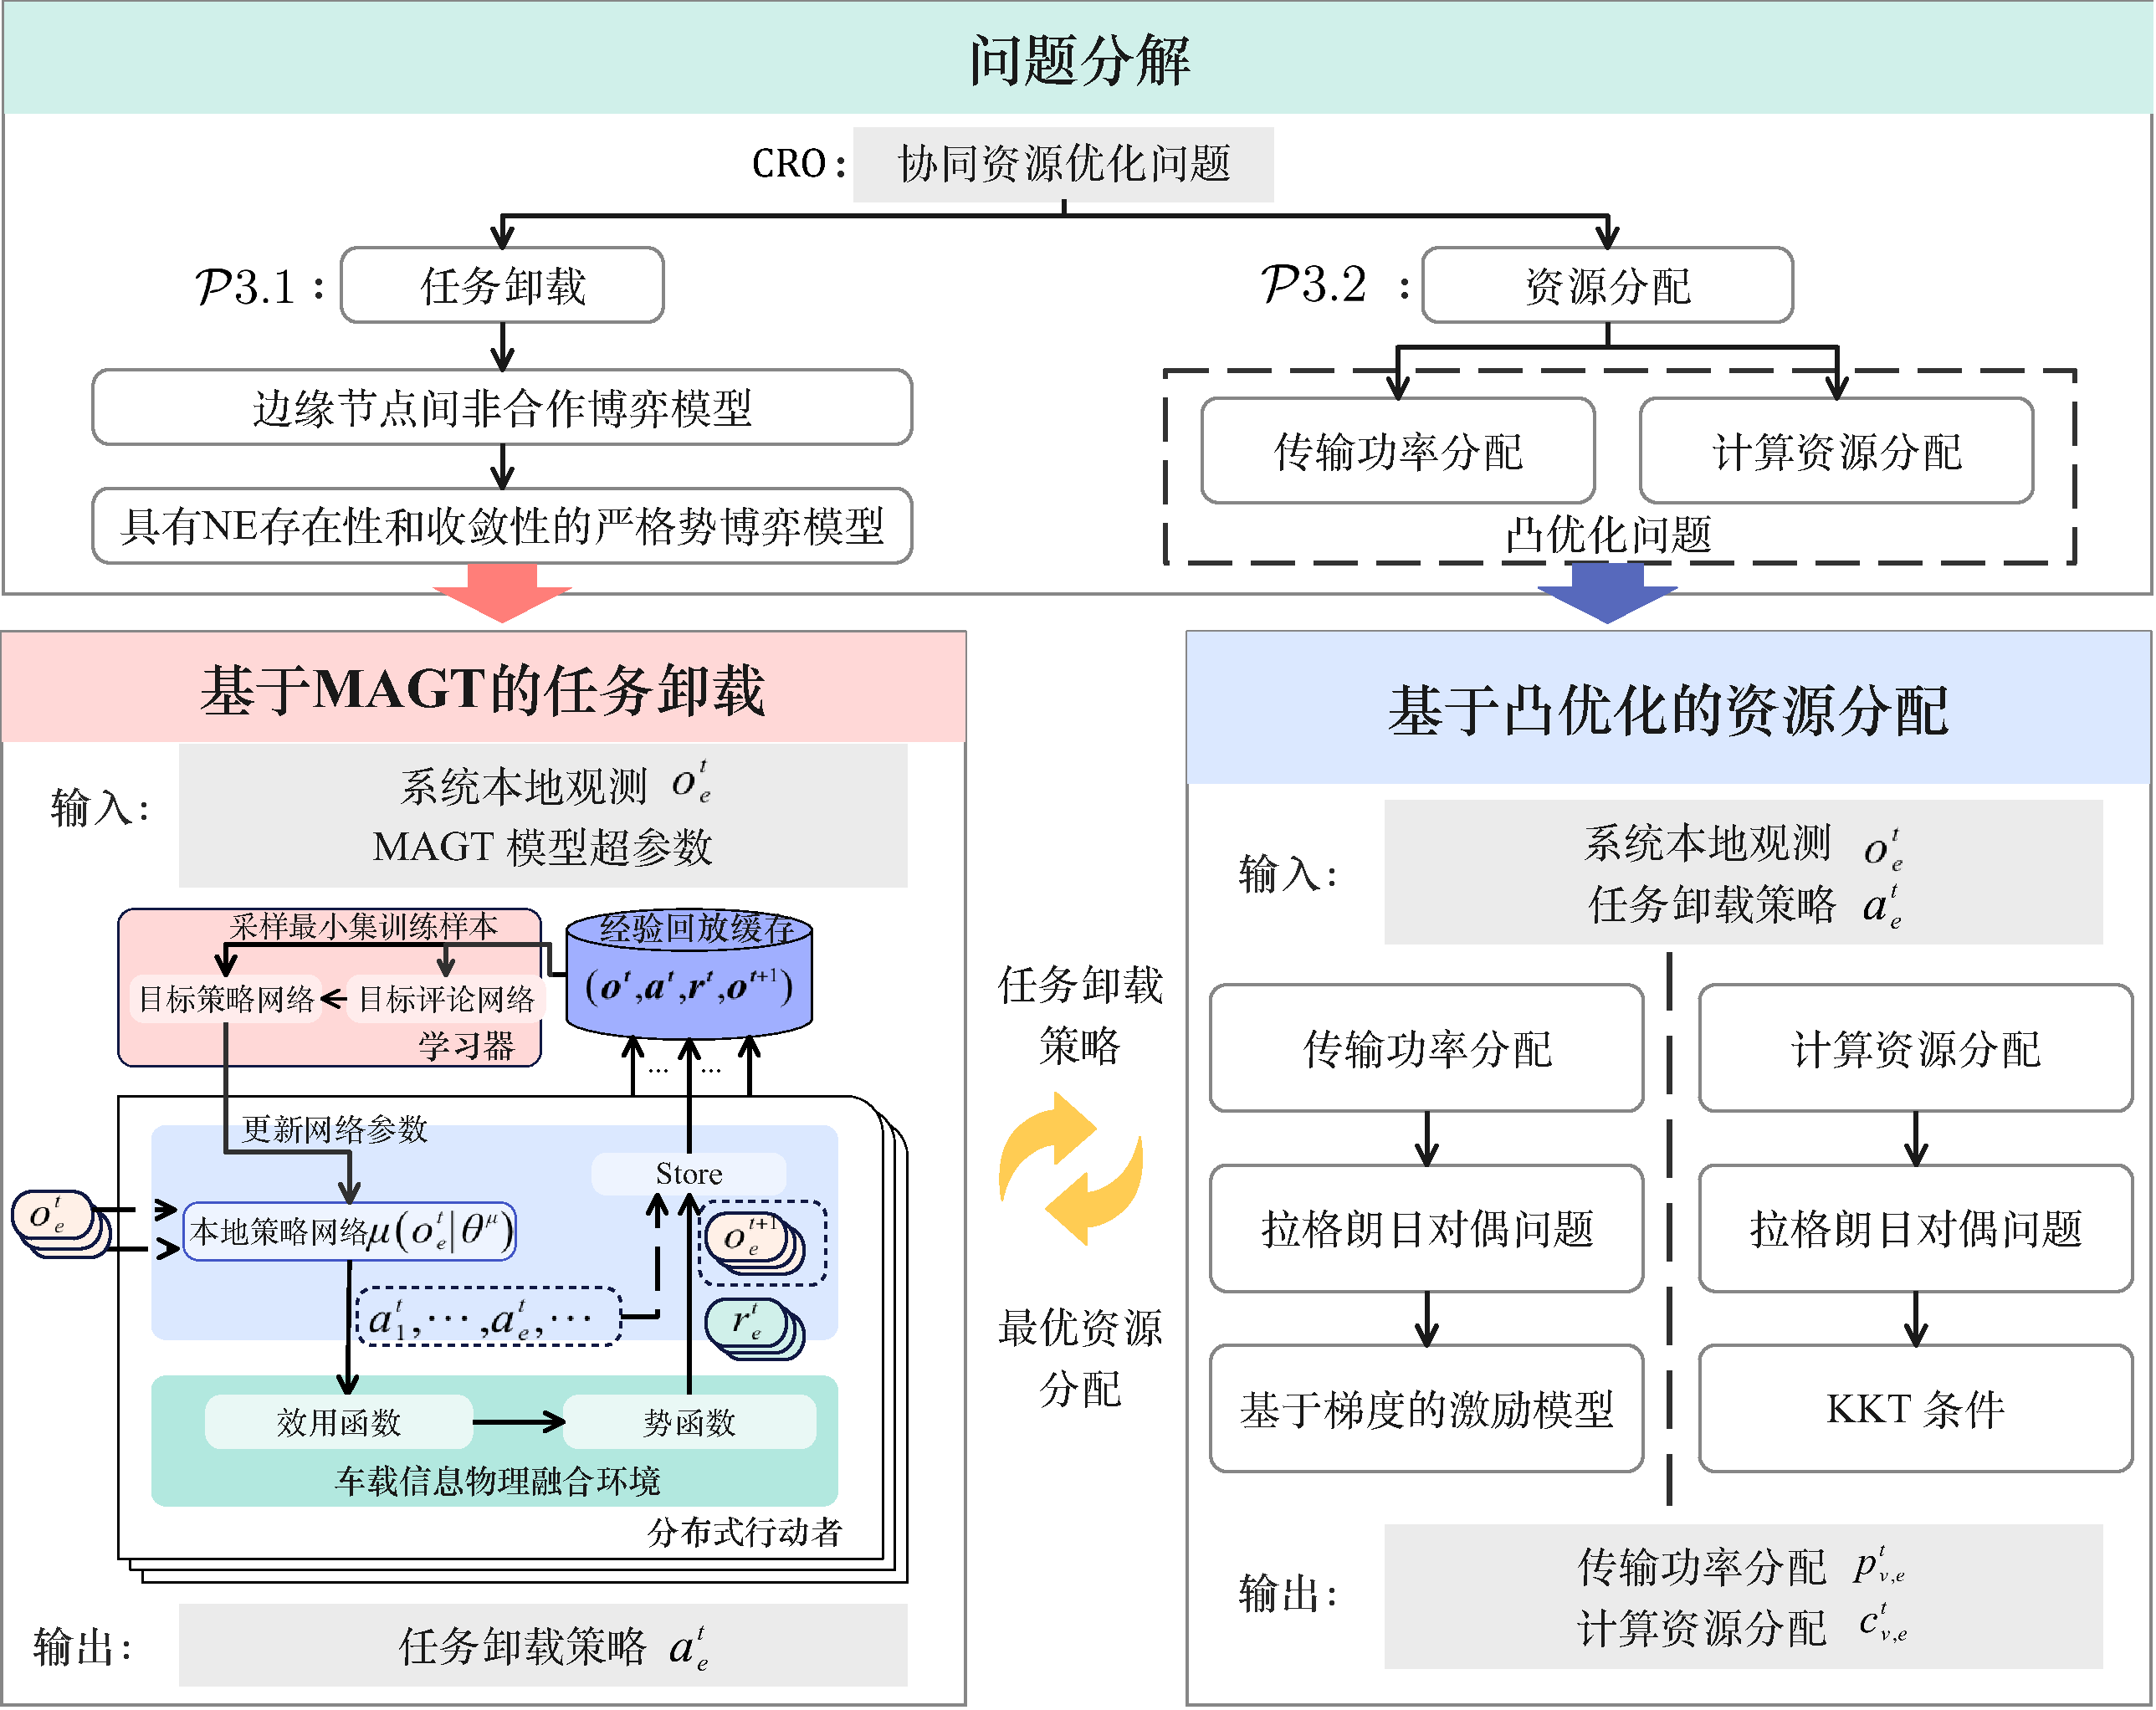
\includegraphics[width=0.3\textwidth]{fig/Fig3-3-solution-model.pdf}
\end{figure}
\end{textblock*}
\end{center}
\end{frame}

\begin{frame}
\frametitle{\englishfont \underline{问题}:协同通信与计算卸载场景}
\newBackground
\begin{center}
\begin{textblock*}{\textwidth}(5.2cm,2.4cm)
\begin{figure}
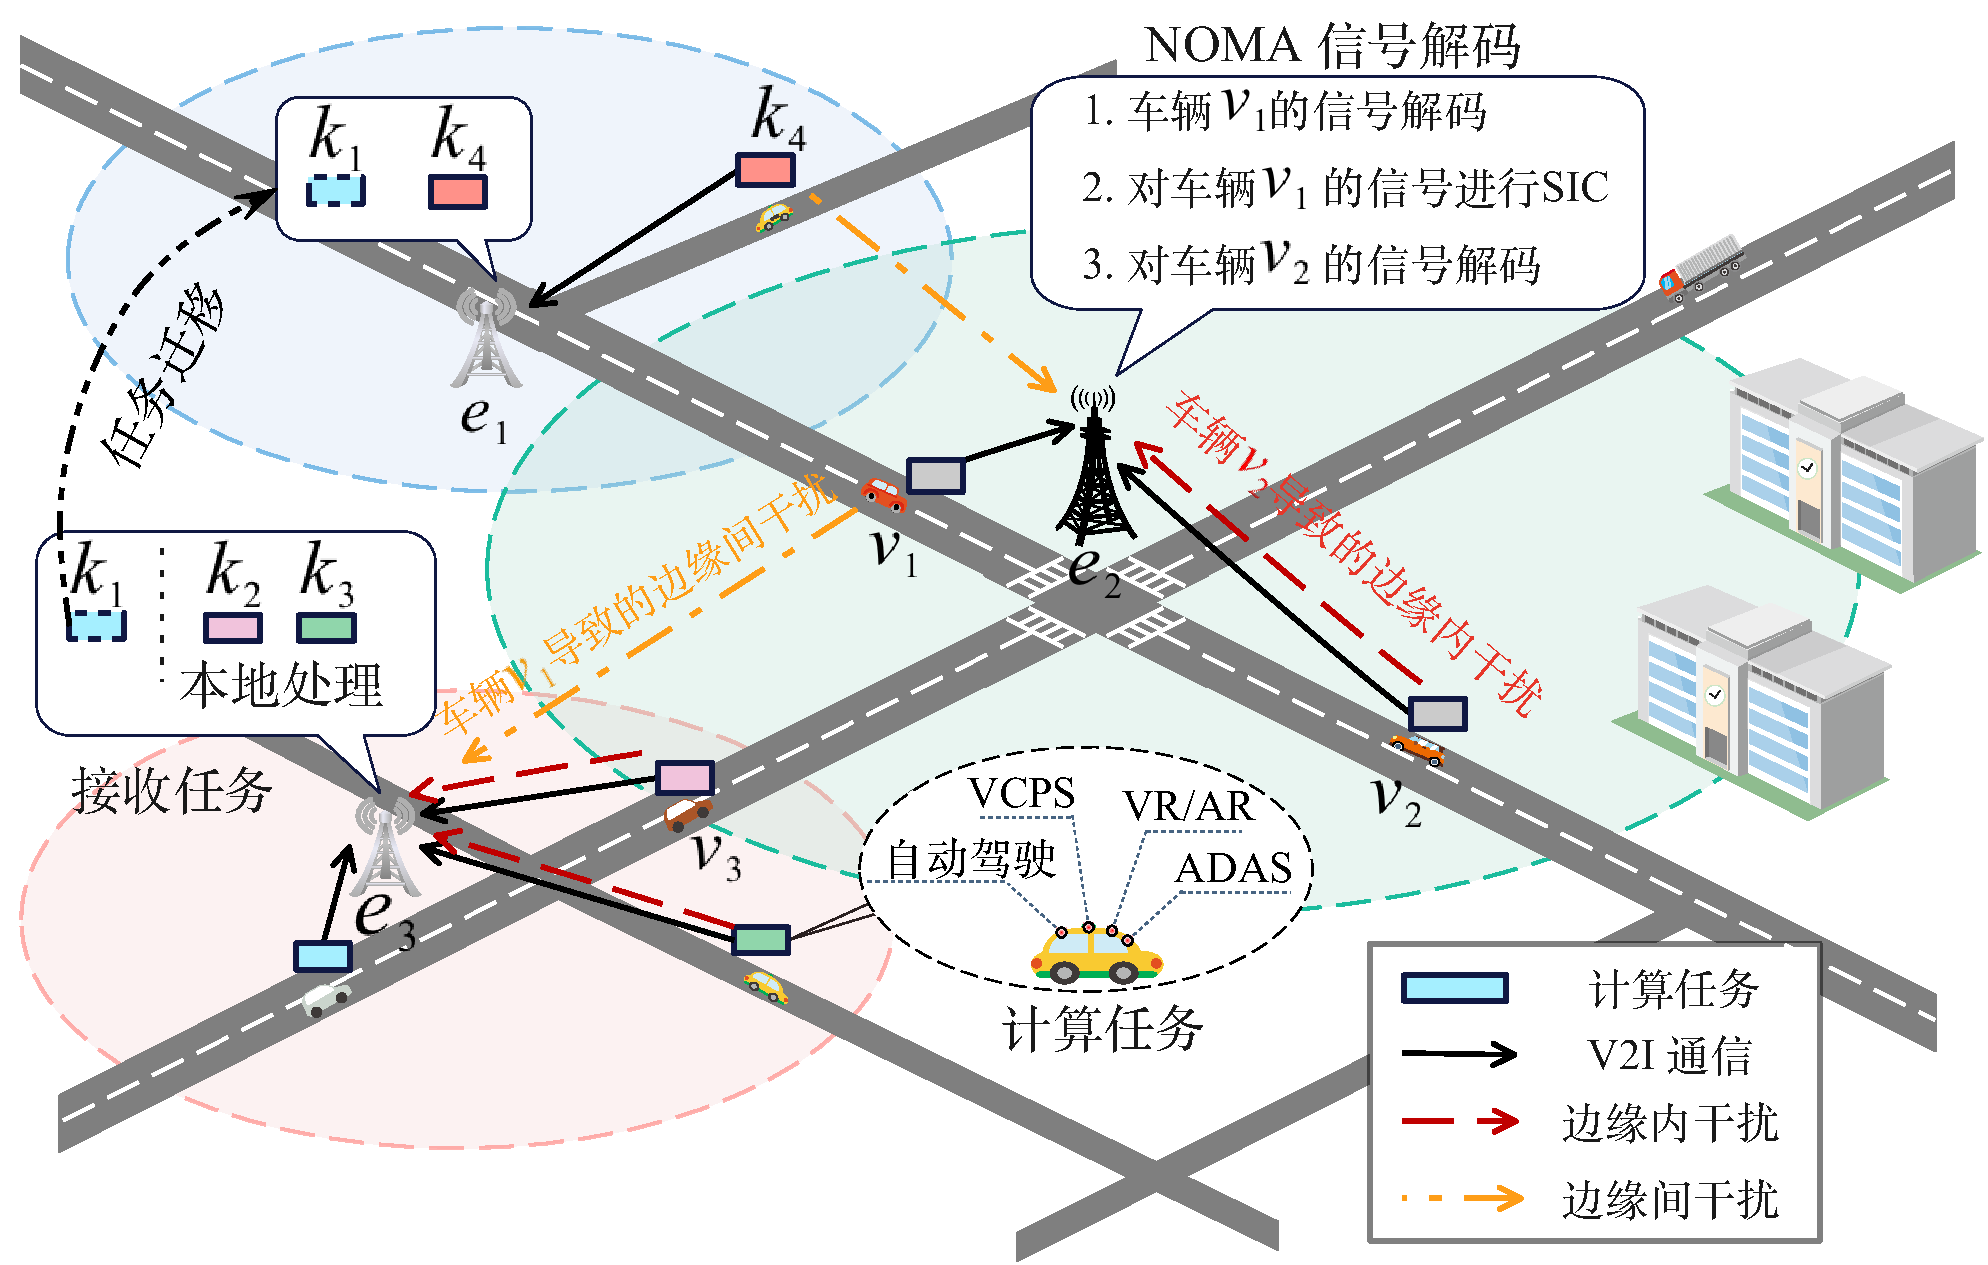
\includegraphics[width=0.55\textwidth]{fig/Fig3-1-noma-architecture.pdf}
\end{figure}
\end{textblock*}
\end{center}

\begin{center}
\begin{textblock*}{\textwidth}(0.5cm,1.8cm)
\begin{itemize}[itemsep=0.2\baselineskip] \englishfont
	\item[\ding{111}] {\color{cqublue}{工作流程}}
	\begin{itemize}[itemsep=0.2\baselineskip]
	\begin{small}
		\item[\ding{226}] \underline{计算任务产生}:车辆随机产生
		\item[\ding{226}] \underline{任务数据上传}:传输功率分配
		\begin{itemize}[itemsep=0.2\baselineskip]
		\footnotesize
			\item[\ding{61}] 车端:叠加编码
			\item[\ding{61}] 边缘端:串行干扰消除
		\end{itemize}
		\item[\ding{226}] \underline{任务本地处理/迁移}:计算资源分配
	\end{small}
	\end{itemize}
	\item[\ding{111}]  {\color{cqublue}{例子}}
	\begin{itemize}[itemsep=0.2\baselineskip]
	\begin{small}
		\item[\ding{226}] 边缘内/边缘间干扰
			\begin{itemize} \footnotesize
				\item[\ding{61}] 边缘内干扰:车辆$v_1$
				\item[\ding{61}] 边缘间干扰:车辆$v_3$
			\end{itemize}
		\item[\ding{226}] 任务负载不匀
		\begin{itemize} \footnotesize
			\item[\ding{61}] 边缘节点$e_3$ (任务$k_1$、$k_2$和$k_3$)$e_1$ (任务$k_4$)
		\end{itemize}
		\item 
	\end{small} 
	\end{itemize}
\end{itemize}
\end{textblock*}
\end{center}
\end{frame}

\begin{frame}
\frametitle{\englishfont \underline{问题}:V2I传输与任务卸载模型}
\newBackground

\begin{overlayarea}{\textwidth}{3cm}

\only<1-1>{
\begin{center}
\begin{textblock*}{1\textwidth}(-3.2cm,1.8cm)
\small	
\begin{equation}
	m_{v, e}^{t} = \frac{d_{k}}{b  \log _{2}\left(1+\mathrm{SINR}_{v, e}^t\right)} \notag
\end{equation}	
\end{textblock*}
\end{center}
}

\only<2-2>{
\begin{center}
\begin{textblock*}{1\textwidth}(-3.2cm,1.8cm)	
\small	
\begin{equation}
	m_{v, e}^{t} = \frac{d_{k}}{b  \log _{2}\left(1+{\color{red}{\mathrm{SINR}_{v, e}^t}}\right)} \notag
\end{equation}	
\end{textblock*}
\end{center}
}

\only<3->{
\begin{center}
\begin{textblock*}{1\textwidth}(-3.2cm,1.8cm)	
\small	
\begin{equation}
	m_{v, e}^{t} = \frac{d_{k}}{b  \log _{2}\left(1+\mathrm{SINR}_{v, e}^t\right)} \notag
\end{equation}	
\end{textblock*}
\end{center}
}

\only<2-2>{
\begin{center}
\begin{textblock*}{1\textwidth}(0.6cm,3.2cm)
\small
{\color{red}{$\mathrm{SINR}_{v, e}^t$}}: 信干噪比
$\mathrm{SINR}_{v, e}^t = \frac{ |h_{v, e}^t| ^{2}  p_{v, e}^{t}}{ \underbrace{\sum\limits_{\forall v^{\prime} \in \mathbf{V}_{h_{v, e}}^{t}} |h_{v^{\prime}, e}^t|^2 p_{v^{\prime}, e}^{t}}_{\text {边缘内干扰}} + \underbrace{\sum\limits_{\forall e^{\prime} \in \mathbf{E} / \{e\}} \sum\limits_{\forall v^{\prime} \in \mathbf{V}_{e^{\prime}}^{t}} |h_{v^{\prime}, e}^t|^2 p_{v^{\prime}, e^{\prime}}^{t}}_{\text {边缘间干扰}} + N_{0}}$
\end{textblock*}
\end{center}
}


\only<1-2>{
\begin{center}
\begin{textblock*}{1\textwidth}(-3.2cm,4.2cm)
\small	
\begin{equation}
	n_{v, e}^t= w_{v, e}^{t} + \sum_{\forall e^{\prime} \in \mathbf{E}} q_{v, e^{\prime}}^{t} x_{v, e^{\prime}}^t \notag
\end{equation}	
\end{textblock*}
\end{center}
}

\only<3-3>{
\begin{center}
\begin{textblock*}{1\textwidth}(-3.2cm,4.2cm)
\small	
\begin{equation}
	n_{v, e}^t= {\color{red}{w_{v, e}^{t}}} + \sum_{\forall e^{\prime} \in \mathbf{E}} q_{v, e^{\prime}}^{t} x_{v, e^{\prime}}^t \notag
\end{equation}	
\end{textblock*}
\end{center}
}

\only<3-3>{
\begin{center}
\begin{textblock*}{1\textwidth}(1.6cm,4.8cm)
\small
{\color{red}{$w_{v, e}^{t}$}}:有线传输时间
\begin{numcases}{w_{v, e}^{t} =}
0, &$k_{v}^{t} \in \mathbf{K}_{e}^{t} \bigcap \mathbf{K}_{q_e}^{t}$ \notag \\
{d_{k}  \operatorname{dis}_{e, e^{\prime}}^{t}}  \zeta  / {z},  &$k_{v}^{t} \in \mathbf{K}_{e}^{t} \bigcap \mathbf{K}_{q_{e^{\prime}}}^{t}$ \notag
\end{numcases}
\end{textblock*}
\end{center}
}

\only<4-4>{
\begin{center}
\begin{textblock*}{1\textwidth}(-3.2cm,4.2cm)
\small	
\begin{equation}
	n_{v, e}^t= w_{v, e}^{t} + \sum_{\forall e^{\prime} \in \mathbf{E}} q_{v, e^{\prime}}^{t} {\color{red}{x_{v, e^{\prime}}^t}} \notag
\end{equation}	
\end{textblock*}
\end{center}
}

\only<4-4>{
\begin{center}
\begin{textblock*}{1\textwidth}(1.6cm,4.6cm)
\small
{\color{red}{$x_{v, e^{\prime}}^t$}}:执行时间
$x_{v, e}^t = \frac{ d_{k}  c_{k}}{c_{v, e}^t}$	
\end{textblock*}
\end{center}
}

\only<5->{
\begin{center}
\begin{textblock*}{1\textwidth}(-3.2cm,4.2cm)
\small	
\begin{equation}
	n_{v, e}^t= w_{v, e}^{t} + \sum_{\forall e^{\prime} \in \mathbf{E}} q_{v, e^{\prime}}^{t} x_{v, e^{\prime}}^t \notag
\end{equation}	
\end{textblock*}
\end{center}
}
\end{overlayarea}



\begin{center}
\begin{textblock*}{1\textwidth}(1cm,1.6cm)
\begin{itemize} \englishfont 
	\item[\ding{111}]  {\color{cqublue}{任务上传时间}}
	\item
	\item 
	\item 
	\item[\ding{111}]  {\color{cqublue}{任务处理时间}}
	\item
	\item
	\item 
	\item 
	\item<5->[\ding{111}]  {\color{cqublue}{任务服务时间}}
	\item<5-> $\psi_{v, e}^{t} = m_{v, e}^{t} +  n_{v, e}^{t}$
\end{itemize}
\end{textblock*}
\end{center}

\end{frame}

\begin{frame}
\frametitle{\englishfont \underline{问题}:协作资源优化 (CRO) 问题}
\newBackground

\begin{overlayarea}{\textwidth}{3cm}
\only<1-1>{
\begin{center}
\begin{textblock*}{1\textwidth}(0.5cm,1.6cm)
\begin{align}
\operatorname{CRO}:&\max_{\mathbf{P}, \mathbf{Q}, \mathbf{C}} f_1= \sum_{\forall t \in \mathbf{T}} \sum_{ \forall e \in \mathbf{E}} \Psi_{e}^{t} \notag \\
		\text { s.t. }
    &\mathcal{C}3.1: \sum_{\forall v \in \mathbf{V}_{e}^{t}} p_{v, e}^{t} \leq p_{e}, \forall e \in \mathbf{E}, \forall t \in \mathbf{T} \notag \\
    &\mathcal{C}3.2: \sum_{\forall k_{v}^{t} \in {\mathbf{K}_{q_e}^{t} }} c_{v, e}^t \leq c_{e}, \forall e \in \mathbf{E}, \forall t \in \mathbf{T} \notag \\
   	&\mathcal{C}3.3: q_{v, e}^t \in \left \{0, 1\right \}, \forall v \in \mathbf{V}, \forall e \in \mathbf{E}, \forall t \in \mathbf{T}  \notag \\
    &\mathcal{C}3.4: \sum_{\forall e \in \mathbf{E}} q_{v, e}^t = 1, \forall v \in \mathbf{V}, \forall t \in \mathbf{T} \notag 
\end{align}
\end{textblock*}
\end{center}
}

\only<2-2>{
\begin{center}
\begin{textblock*}{1\textwidth}(0.5cm,1.6cm)
\begin{align}
\operatorname{CRO}:&\max_{\mathbf{P}, \mathbf{Q}, \mathbf{C}} f_1= \sum_{\forall t \in \mathbf{T}} \sum_{ \forall e \in \mathbf{E}} {\color{red}{\Psi_{e}^{t}}} \notag \\
		\text { s.t. }
    &\mathcal{C}3.1: \sum_{\forall v \in \mathbf{V}_{e}^{t}} p_{v, e}^{t} \leq p_{e}, \forall e \in \mathbf{E}, \forall t \in \mathbf{T} \notag \\
    &\mathcal{C}3.2: \sum_{\forall k_{v}^{t} \in {\mathbf{K}_{q_e}^{t} }} c_{v, e}^t \leq c_{e}, \forall e \in \mathbf{E}, \forall t \in \mathbf{T} \notag \\
   	&\mathcal{C}3.3: q_{v, e}^t \in \left \{0, 1\right \}, \forall v \in \mathbf{V}, \forall e \in \mathbf{E}, \forall t \in \mathbf{T}  \notag \\
    &\mathcal{C}3.4: \sum_{\forall e \in \mathbf{E}} q_{v, e}^t = 1, \forall v \in \mathbf{V}, \forall t \in \mathbf{T} \notag 
\end{align}
\end{textblock*}
\end{center}
}

\only<2-2>{
\begin{center}
\begin{textblock*}{1\textwidth}(0.5cm,7.1cm) \englishfont
{\color{red}{$\Psi_{e}^{t}$}}:服务率 $\Psi_{e}^{t} = \frac{\sum_{\forall k_{v}^{t} \in \mathbf{K}_{e}^{t}} \mathbb{I} \left\{ \psi_{v, e}^{t} \leq t_{k} \right\} }{|\mathbf{K}_{e}^{t}|}$
\end{textblock*}
\end{center}
}


\only<3-3>{
\begin{center}
\begin{textblock*}{1\textwidth}(0.5cm,1.6cm)
\begin{align}
\operatorname{CRO}:&\max_{{\color{red}{\mathbf{P}}}, \mathbf{Q}, \mathbf{C}} f_1= \sum_{\forall t \in \mathbf{T}} \sum_{ \forall e \in \mathbf{E}} \Psi_{e}^{t} \notag \\
		\text { s.t. }
    &\mathcal{C}3.1: \sum_{\forall v \in \mathbf{V}_{e}^{t}} p_{v, e}^{t} \leq p_{e}, \forall e \in \mathbf{E}, \forall t \in \mathbf{T} \notag \\
    &\mathcal{C}3.2: \sum_{\forall k_{v}^{t} \in {\mathbf{K}_{q_e}^{t} }} c_{v, e}^t \leq c_{e}, \forall e \in \mathbf{E}, \forall t \in \mathbf{T} \notag \\
   	&\mathcal{C}3.3: q_{v, e}^t \in \left \{0, 1\right \}, \forall v \in \mathbf{V}, \forall e \in \mathbf{E}, \forall t \in \mathbf{T}  \notag \\
    &\mathcal{C}3.4: \sum_{\forall e \in \mathbf{E}} q_{v, e}^t = 1, \forall v \in \mathbf{V}, \forall t \in \mathbf{T} \notag 
\end{align}
\end{textblock*}
\end{center}
}

\only<3-3>{
\begin{center}
\begin{textblock*}{1\textwidth}(0.5cm,7.1cm) \englishfont
{\color{red}{$\mathbf{P}$}}:传输功率分配 $\mathbf{P}= \left \{ p_{v, e}^{t} \mid \forall v \in \mathbf{V}_{e}^t, \forall e \in \mathbf{E}, \forall t \in \mathbf{T}\right \}$
\end{textblock*}
\end{center}
}

\only<4-4>{
\begin{center}
\begin{textblock*}{1\textwidth}(0.5cm,1.6cm)
\begin{align}
\operatorname{CRO}:&\max_{\mathbf{P}, {\color{red}{\mathbf{Q}}}, \mathbf{C}} f_1= \sum_{\forall t \in \mathbf{T}} \sum_{ \forall e \in \mathbf{E}} \Psi_{e}^{t} \notag \\
		\text { s.t. }
    &\mathcal{C}3.1: \sum_{\forall v \in \mathbf{V}_{e}^{t}} p_{v, e}^{t} \leq p_{e}, \forall e \in \mathbf{E}, \forall t \in \mathbf{T} \notag \\
    &\mathcal{C}3.2: \sum_{\forall k_{v}^{t} \in {\mathbf{K}_{q_e}^{t} }} c_{v, e}^t \leq c_{e}, \forall e \in \mathbf{E}, \forall t \in \mathbf{T} \notag \\
   	&\mathcal{C}3.3: q_{v, e}^t \in \left \{0, 1\right \}, \forall v \in \mathbf{V}, \forall e \in \mathbf{E}, \forall t \in \mathbf{T}  \notag \\
    &\mathcal{C}3.4: \sum_{\forall e \in \mathbf{E}} q_{v, e}^t = 1, \forall v \in \mathbf{V}, \forall t \in \mathbf{T} \notag 
\end{align}
\end{textblock*}
\end{center}
}

\only<4-4>{
\begin{center}
\begin{textblock*}{1\textwidth}(0.5cm,7.1cm) \englishfont
{\color{red}{$\mathbf{Q}$}}:任务卸载决策 $\mathbf{Q}= \left \{ q_{v, e}^t \mid \forall v \in \mathbf{V}, \forall e \in \mathbf{E}, \forall t \in \mathbf{T} \right \}$
\end{textblock*}
\end{center}
}

\only<5-5>{
\begin{center}
\begin{textblock*}{1\textwidth}(0.5cm,1.6cm)
\begin{align}
\operatorname{CRO}:&\max_{\mathbf{P}, \mathbf{Q}, {\color{red}{\mathbf{C}}}} f_1= \sum_{\forall t \in \mathbf{T}} \sum_{ \forall e \in \mathbf{E}} \Psi_{e}^{t} \notag \\
		\text { s.t. }
    &\mathcal{C}3.1: \sum_{\forall v \in \mathbf{V}_{e}^{t}} p_{v, e}^{t} \leq p_{e}, \forall e \in \mathbf{E}, \forall t \in \mathbf{T} \notag \\
    &\mathcal{C}3.2: \sum_{\forall k_{v}^{t} \in {\mathbf{K}_{q_e}^{t} }} c_{v, e}^t \leq c_{e}, \forall e \in \mathbf{E}, \forall t \in \mathbf{T} \notag \\
   	&\mathcal{C}3.3: q_{v, e}^t \in \left \{0, 1\right \}, \forall v \in \mathbf{V}, \forall e \in \mathbf{E}, \forall t \in \mathbf{T}  \notag \\
    &\mathcal{C}3.4: \sum_{\forall e \in \mathbf{E}} q_{v, e}^t = 1, \forall v \in \mathbf{V}, \forall t \in \mathbf{T} \notag 
\end{align}
\end{textblock*}
\end{center}
}

\only<5-5>{
\begin{center}
\begin{textblock*}{1\textwidth}(0.5cm,7.1cm) \englishfont
{\color{red}{$\mathbf{C}$}}:计算资源分配 $\mathbf{C}= \left \{ c_{v, e}^t \mid \forall v \in \mathbf{V}, \forall e \in \mathbf{E}, \forall t \in \mathbf{T} \right \}$
\end{textblock*}
\end{center}
}

\only<6-6>{
\begin{center}
\begin{textblock*}{1\textwidth}(0.5cm,1.6cm)
\begin{align}
\operatorname{CRO}:&\max_{\mathbf{P}, \mathbf{Q}, \mathbf{C}} f_1= \sum_{\forall t \in \mathbf{T}} \sum_{ \forall e \in \mathbf{E}} \Psi_{e}^{t} \notag \\
		\text { s.t. }
    &{\color{red}{\mathcal{C}3.1}}: \sum_{\forall v \in \mathbf{V}_{e}^{t}} p_{v, e}^{t} \leq p_{e}, \forall e \in \mathbf{E}, \forall t \in \mathbf{T} \notag \\
    &\mathcal{C}3.2: \sum_{\forall k_{v}^{t} \in {\mathbf{K}_{q_e}^{t} }} c_{v, e}^t \leq c_{e}, \forall e \in \mathbf{E}, \forall t \in \mathbf{T} \notag \\
   	&\mathcal{C}3.3: q_{v, e}^t \in \left \{0, 1\right \}, \forall v \in \mathbf{V}, \forall e \in \mathbf{E}, \forall t \in \mathbf{T}  \notag \\
    &\mathcal{C}3.4: \sum_{\forall e \in \mathbf{E}} q_{v, e}^t = 1, \forall v \in \mathbf{V}, \forall t \in \mathbf{T} \notag 
\end{align}
\end{textblock*}
\end{center}
}

\only<6-6>{
\begin{center}
\begin{textblock*}{1\textwidth}(0.5cm,7.1cm) \englishfont
{\color{red}{$\mathcal{C}3.1$}}:边缘节点分配的总传输功率不能超过V2I通信的最大功率
\end{textblock*}
\end{center}
}

\only<7-7>{
\begin{center}
\begin{textblock*}{1\textwidth}(0.5cm,1.6cm)
\begin{align}
\operatorname{CRO}:&\max_{\mathbf{P}, \mathbf{Q}, \mathbf{C}} f_1= \sum_{\forall t \in \mathbf{T}} \sum_{ \forall e \in \mathbf{E}} \Psi_{e}^{t} \notag \\
		\text { s.t. }
    &\mathcal{C}3.1: \sum_{\forall v \in \mathbf{V}_{e}^{t}} p_{v, e}^{t} \leq p_{e}, \forall e \in \mathbf{E}, \forall t \in \mathbf{T} \notag \\
    &{\color{red}{\mathcal{C}3.2}}: \sum_{\forall k_{v}^{t} \in {\mathbf{K}_{q_e}^{t} }} c_{v, e}^t \leq c_{e}, \forall e \in \mathbf{E}, \forall t \in \mathbf{T} \notag \\
   	&\mathcal{C}3.3: q_{v, e}^t \in \left \{0, 1\right \}, \forall v \in \mathbf{V}, \forall e \in \mathbf{E}, \forall t \in \mathbf{T}  \notag \\
    &\mathcal{C}3.4: \sum_{\forall e \in \mathbf{E}} q_{v, e}^t = 1, \forall v \in \mathbf{V}, \forall t \in \mathbf{T} \notag 
\end{align}
\end{textblock*}
\end{center}
}

\only<7-7>{
\begin{center}
\begin{textblock*}{1\textwidth}(0.5cm,7.1cm) \englishfont
{\color{red}{$\mathcal{C}2.2$}}:分配的总体计算资源不能超过边缘节点的计算能力
\end{textblock*}
\end{center}
}

\only<8-8>{
\begin{center}
\begin{textblock*}{1\textwidth}(0.5cm,1.6cm)
\begin{align}
\operatorname{CRO}:&\max_{\mathbf{P}, \mathbf{Q}, \mathbf{C}} f_1= \sum_{\forall t \in \mathbf{T}} \sum_{ \forall e \in \mathbf{E}} \Psi_{e}^{t} \notag \\
		\text { s.t. }
    &\mathcal{C}3.1: \sum_{\forall v \in \mathbf{V}_{e}^{t}} p_{v, e}^{t} \leq p_{e}, \forall e \in \mathbf{E}, \forall t \in \mathbf{T} \notag \\
    &\mathcal{C}3.2: \sum_{\forall k_{v}^{t} \in {\mathbf{K}_{q_e}^{t} }} c_{v, e}^t \leq c_{e}, \forall e \in \mathbf{E}, \forall t \in \mathbf{T} \notag \\
   	&{\color{red}{\mathcal{C}3.3}}: q_{v, e}^t \in \left \{0, 1\right \}, \forall v \in \mathbf{V}, \forall e \in \mathbf{E}, \forall t \in \mathbf{T}  \notag \\
    &\mathcal{C}3.4: \sum_{\forall e \in \mathbf{E}} q_{v, e}^t = 1, \forall v \in \mathbf{V}, \forall t \in \mathbf{T} \notag 
\end{align}
\end{textblock*}
\end{center}
}

\only<8-8>{
\begin{center}
\begin{textblock*}{1\textwidth}(0.5cm,7.1cm) \englishfont
{\color{red}{$\mathcal{C}3.3$}}:任务卸载决策是 0-1 变量
\end{textblock*}
\end{center}
}

\only<9-9>{
\begin{center}
\begin{textblock*}{1\textwidth}(0.5cm,1.6cm)
\begin{align}
\operatorname{CRO}:&\max_{\mathbf{P}, \mathbf{Q}, \mathbf{C}} f_1= \sum_{\forall t \in \mathbf{T}} \sum_{ \forall e \in \mathbf{E}} \Psi_{e}^{t} \notag \\
		\text { s.t. }
    &\mathcal{C}3.1: \sum_{\forall v \in \mathbf{V}_{e}^{t}} p_{v, e}^{t} \leq p_{e}, \forall e \in \mathbf{E}, \forall t \in \mathbf{T} \notag \\
    &\mathcal{C}3.2: \sum_{\forall k_{v}^{t} \in {\mathbf{K}_{q_e}^{t} }} c_{v, e}^t \leq c_{e}, \forall e \in \mathbf{E}, \forall t \in \mathbf{T} \notag \\
   	&\mathcal{C}3.3: q_{v, e}^t \in \left \{0, 1\right \}, \forall v \in \mathbf{V}, \forall e \in \mathbf{E}, \forall t \in \mathbf{T}  \notag \\
    &{\color{red}{\mathcal{C}3.4}}: \sum_{\forall e \in \mathbf{E}} q_{v, e}^t = 1, \forall v \in \mathbf{V}, \forall t \in \mathbf{T} \notag 
\end{align}
\end{textblock*}
\end{center}
}

\only<9-9>{
\begin{center}
\begin{textblock*}{1\textwidth}(0.5cm,7.1cm) \englishfont
{\color{red}{$\mathcal{C}3.4$}}:每个任务只能卸载到一个边缘节点
\end{textblock*}
\end{center}
}


\end{overlayarea}
\end{frame}

\begin{frame}
\frametitle{\englishfont \underline{算法}:问题分解}
\newBackground
\begin{center}
\begin{textblock*}{\textwidth}(5.7cm,2.3cm)
\begin{figure}
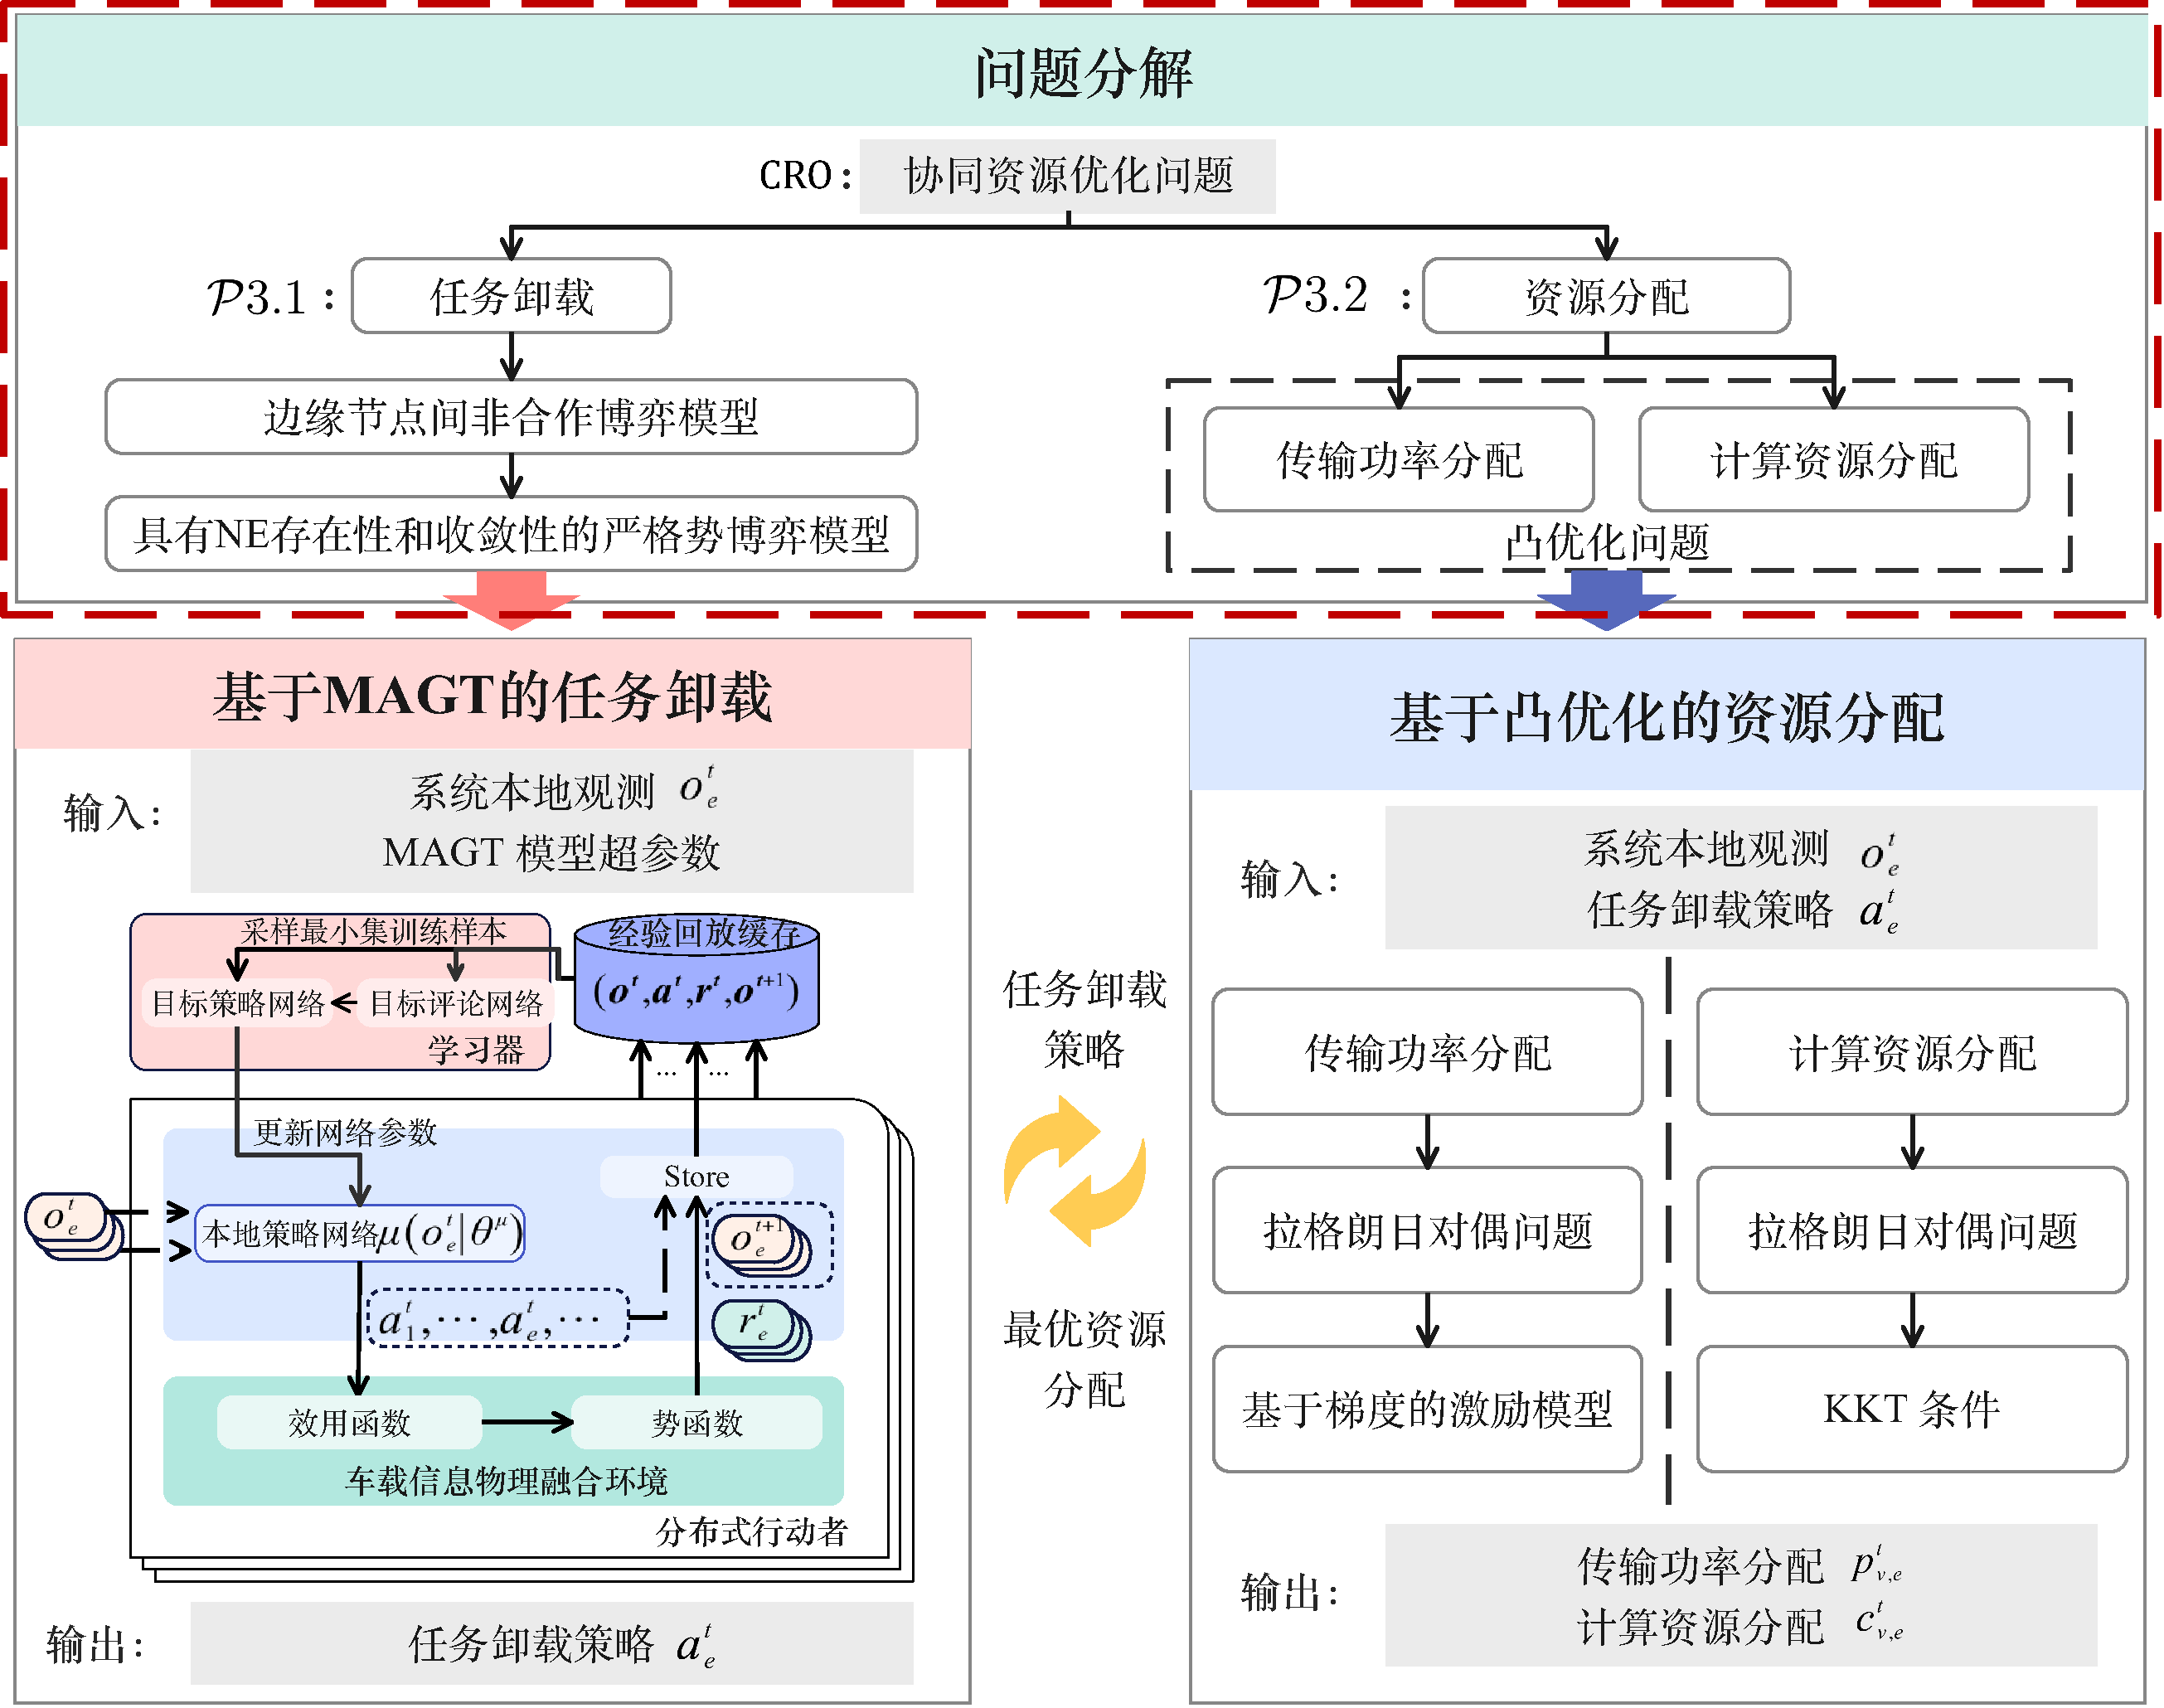
\includegraphics[width=0.45\textwidth]{fig/Fig3-3-solution-model1.pdf}
\end{figure}
\end{textblock*}
\end{center}

\begin{center}
\begin{textblock*}{0.75\textwidth}(0.5cm,2cm)
\begin{itemize}[itemsep=0.2\baselineskip] \englishfont 
	\item[\ding{111}] {\color{cqublue}{任务卸载问题}}
	\begin{itemize}[itemsep=0.2\baselineskip]
	\begin{small}
		\item[\ding{226}] 边缘节点非合作博弈{\small{$\mathcal{G} = \left\{\mathbf{E}, \mathbb{S}, \left\{{U}_{e}\right\}_{\forall e \in \mathbf{E}} \right\}$}}
		\item[\ding{226}] 效用函数{\small{${U}_{e}\left(\mathcal{S}\right) = \sum_{\forall e \in \mathbf{E}} \Psi_{e}^{t}$}}
		\item[\ding{226}] 势函数{\small{${F}_{e}\left(\mathcal{S}\right) = {U}_{e}\left(\mathcal{S}_{e}, \mathcal{S}_{-e}\right) - {U}_{e}\left(-\mathcal{S}_{e}, \mathcal{S}_{-e}\right)$}}
		\item[\ding{226}] 具有NE存在和收敛性的严格势博弈 (EPG)
	\end{small}
	\end{itemize}
	\item[\ding{111}]  {\color{cqublue}{资源分配问题}}
	\begin{itemize}[itemsep=0.2\baselineskip]
	\begin{small}
		\item[\ding{226}] 传输功率分配\\{\small{$ \min_{\mathbf{P}^{t}} \sum_{ \forall e \in \mathbf{E}} \sum_{\forall k_{v}^{t} \in \mathbf{K}_{e}^{t}}  \frac{d_{k}}{b  \log _{2}\left(1+\mathrm{SINR}_{v, e}^t\right)}$}}
		\item[\ding{226}] 计算资源分配\\{\small{$ \min_{\mathbf{C}^{t}} \sum_{ \forall e \in \mathbf{E}} \sum_{\forall k_{v}^{t} \in \mathbf{K}_{e}^{t}} ( w_{v, e}^{t} + \sum_{\forall e^{\prime} \in \mathbf{E}} q_{v, e^{\prime}}^{t} x_{v, e^{\prime}}^t)$}}
	\end{small}
	\end{itemize}
\end{itemize}
\end{textblock*}
\end{center}
\end{frame}

\begin{frame}
\frametitle{\englishfont \underline{算法}:基于MAGT的任务卸载}
\newBackground
\begin{center}
\begin{textblock*}{\textwidth}(5.7cm,2.3cm)
\begin{figure}
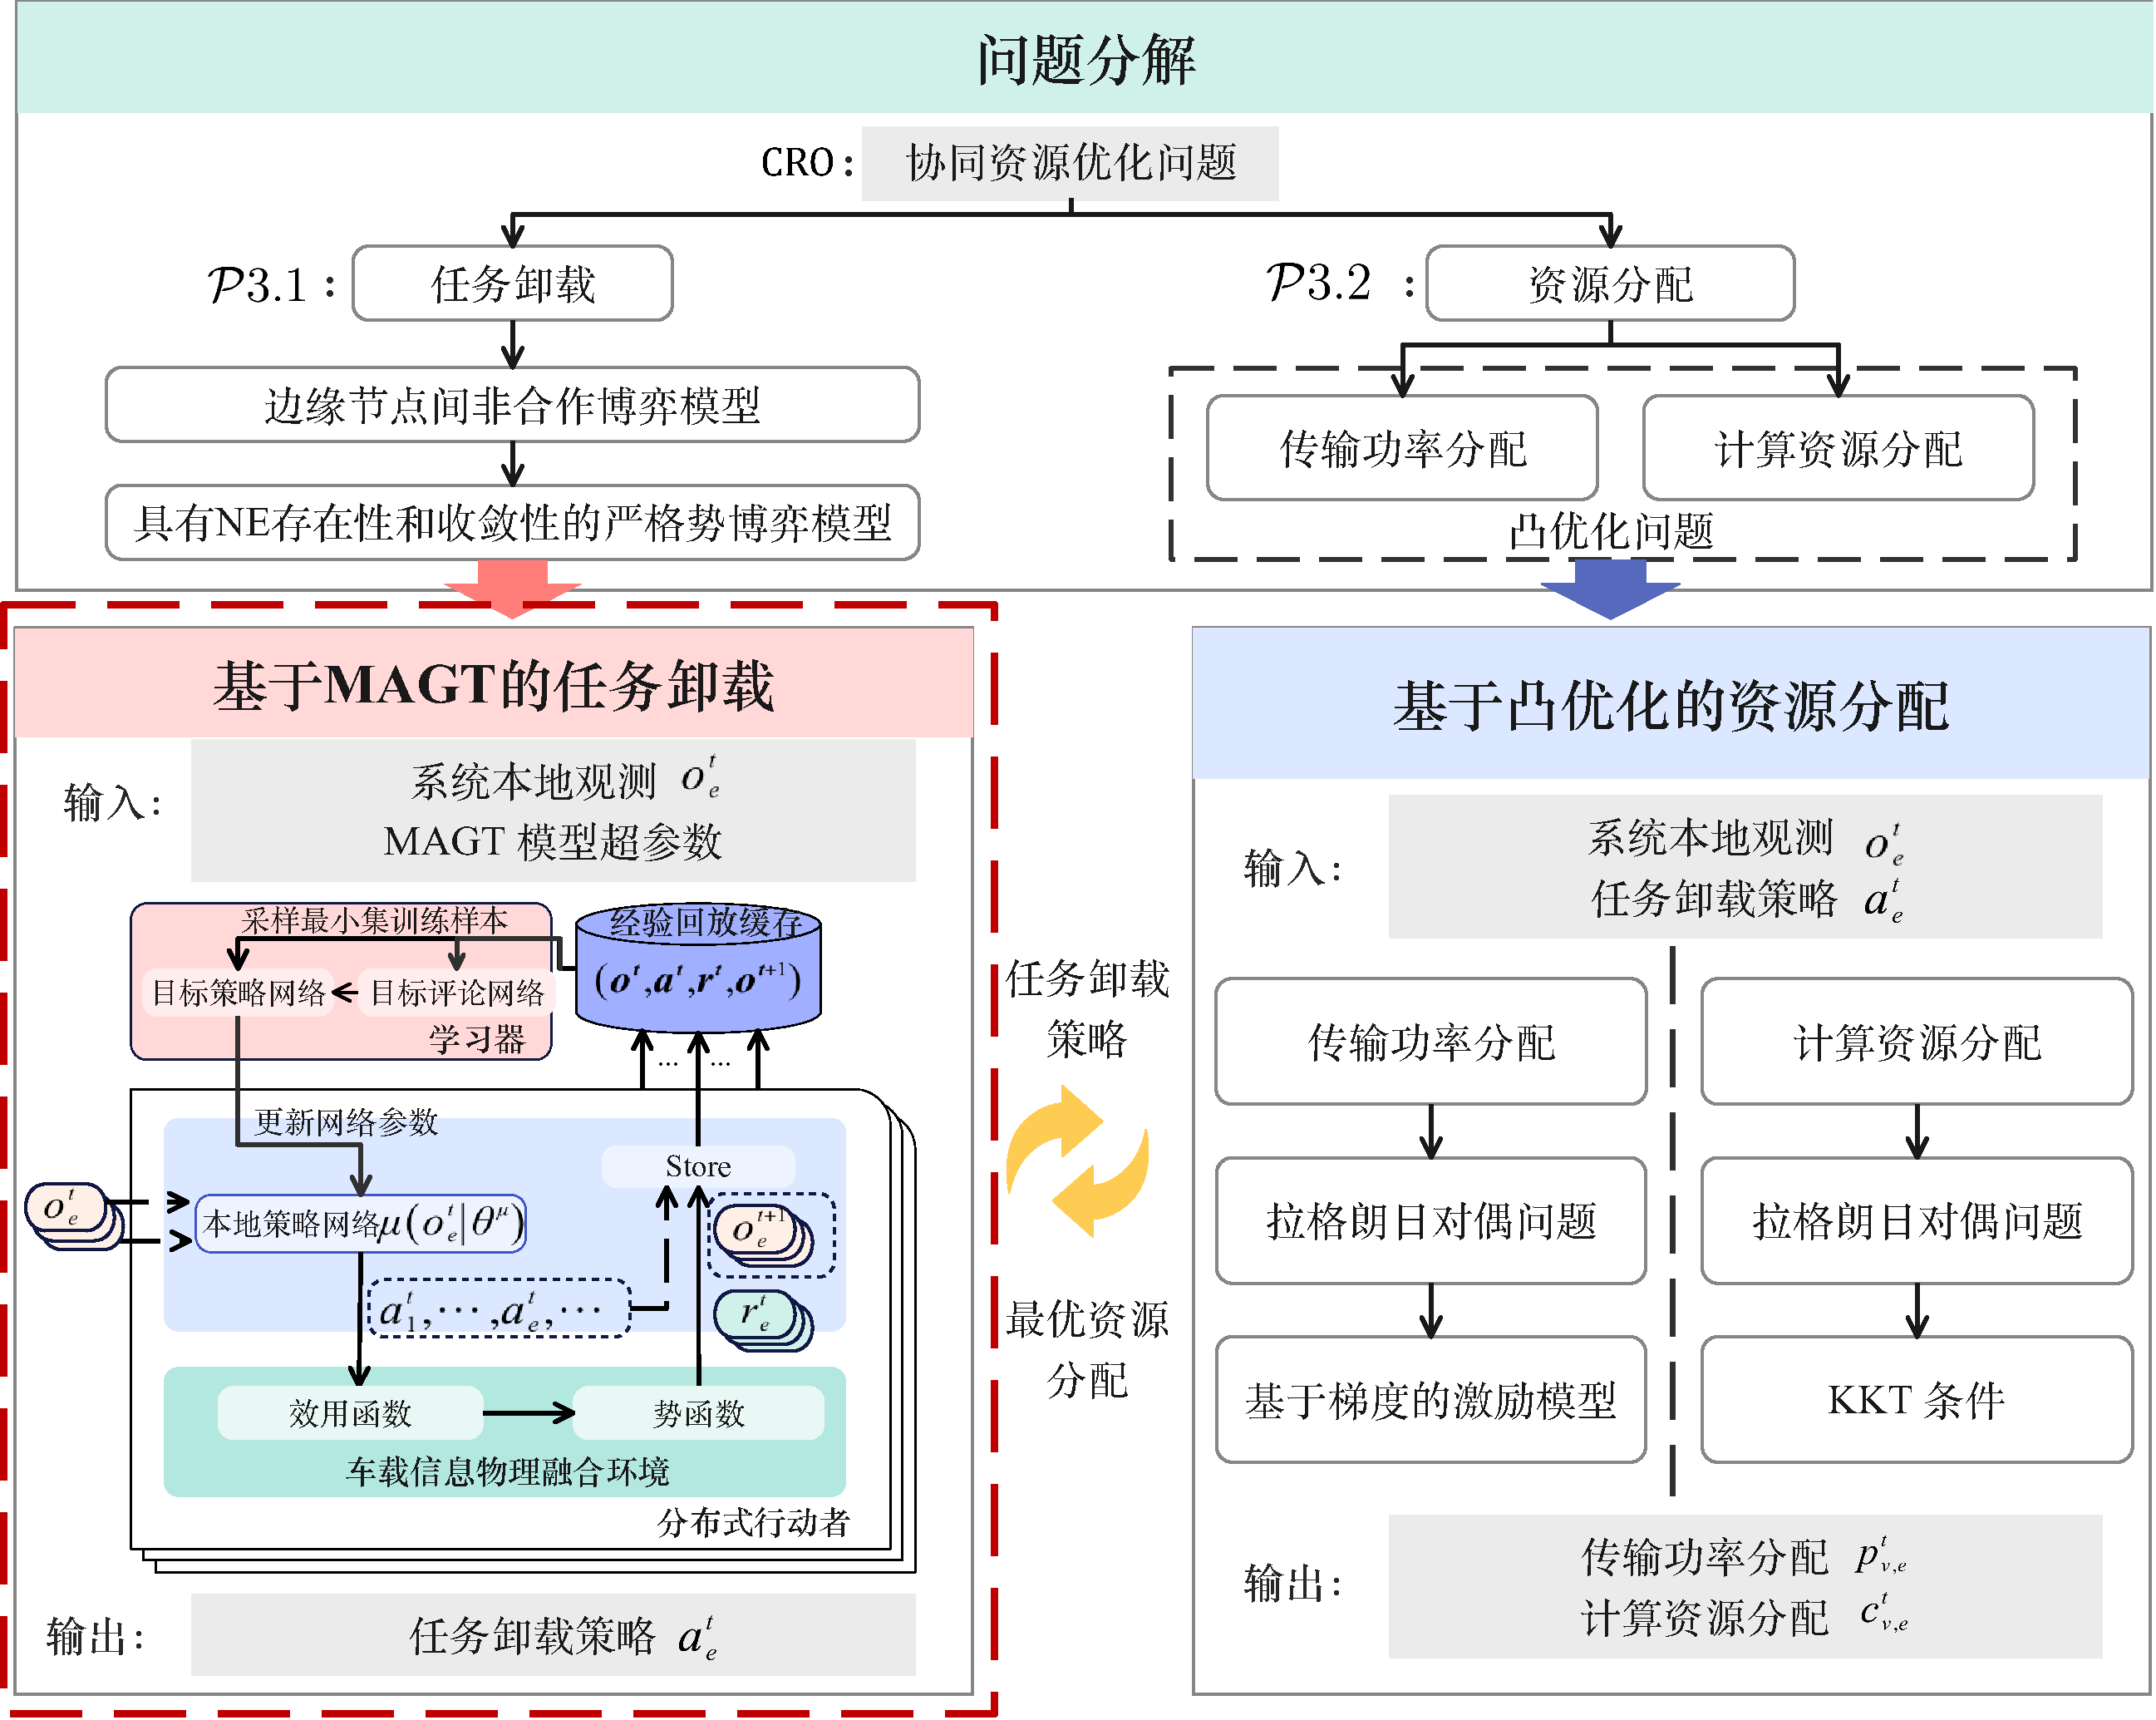
\includegraphics[width=0.45\textwidth]{fig/Fig3-3-solution-model2.pdf}
\end{figure}
\end{textblock*}
\end{center}

\begin{center}
\begin{textblock*}{0.6\textwidth}(0.5cm,2cm)
\begin{itemize} \englishfont
	\item[\ding{111}] {\color{cqublue}{系统状态}}
	\item 边缘节点观测
	\item $\boldsymbol{o}_{e}^{t}=\left\{e, t, \mathbf{Dis}_{\mathbf{V}_{e}^{t}}, \mathbf{D}_{\mathbf{K}_{e}^{t}}, \mathbf{C}_{\mathbf{K}_{e}^{t}}, \mathbf{T}_{\mathbf{K}_{v}^{t}}\right\}$
	\item[\ding{111}] {\color{cqublue}{动作空间}}
	\item 车辆请求任务的卸载决策
	\item $\boldsymbol{a}_{e}^{t} = \left\{ q_{v, e^{\prime}}^t \mid \forall e^{\prime} \in \mathbf{E}, \forall v \in \mathbf{V}_{e}^{t} \right\}$
	\item[\ding{111}] {\color{cqublue}{奖励函数}}
	\item 博弈中效用函数\ding{221}系统奖励函数
	\item 博弈中势函数\ding{221}边缘节点奖励函数
\end{itemize}
\end{textblock*}
\end{center}

\end{frame}

\begin{frame}
\frametitle{\englishfont \underline{算法}:基于凸优化的资源分配}
\newBackground
\begin{center}
\begin{textblock*}{\textwidth}(5.7cm,2.3cm)
\begin{figure}
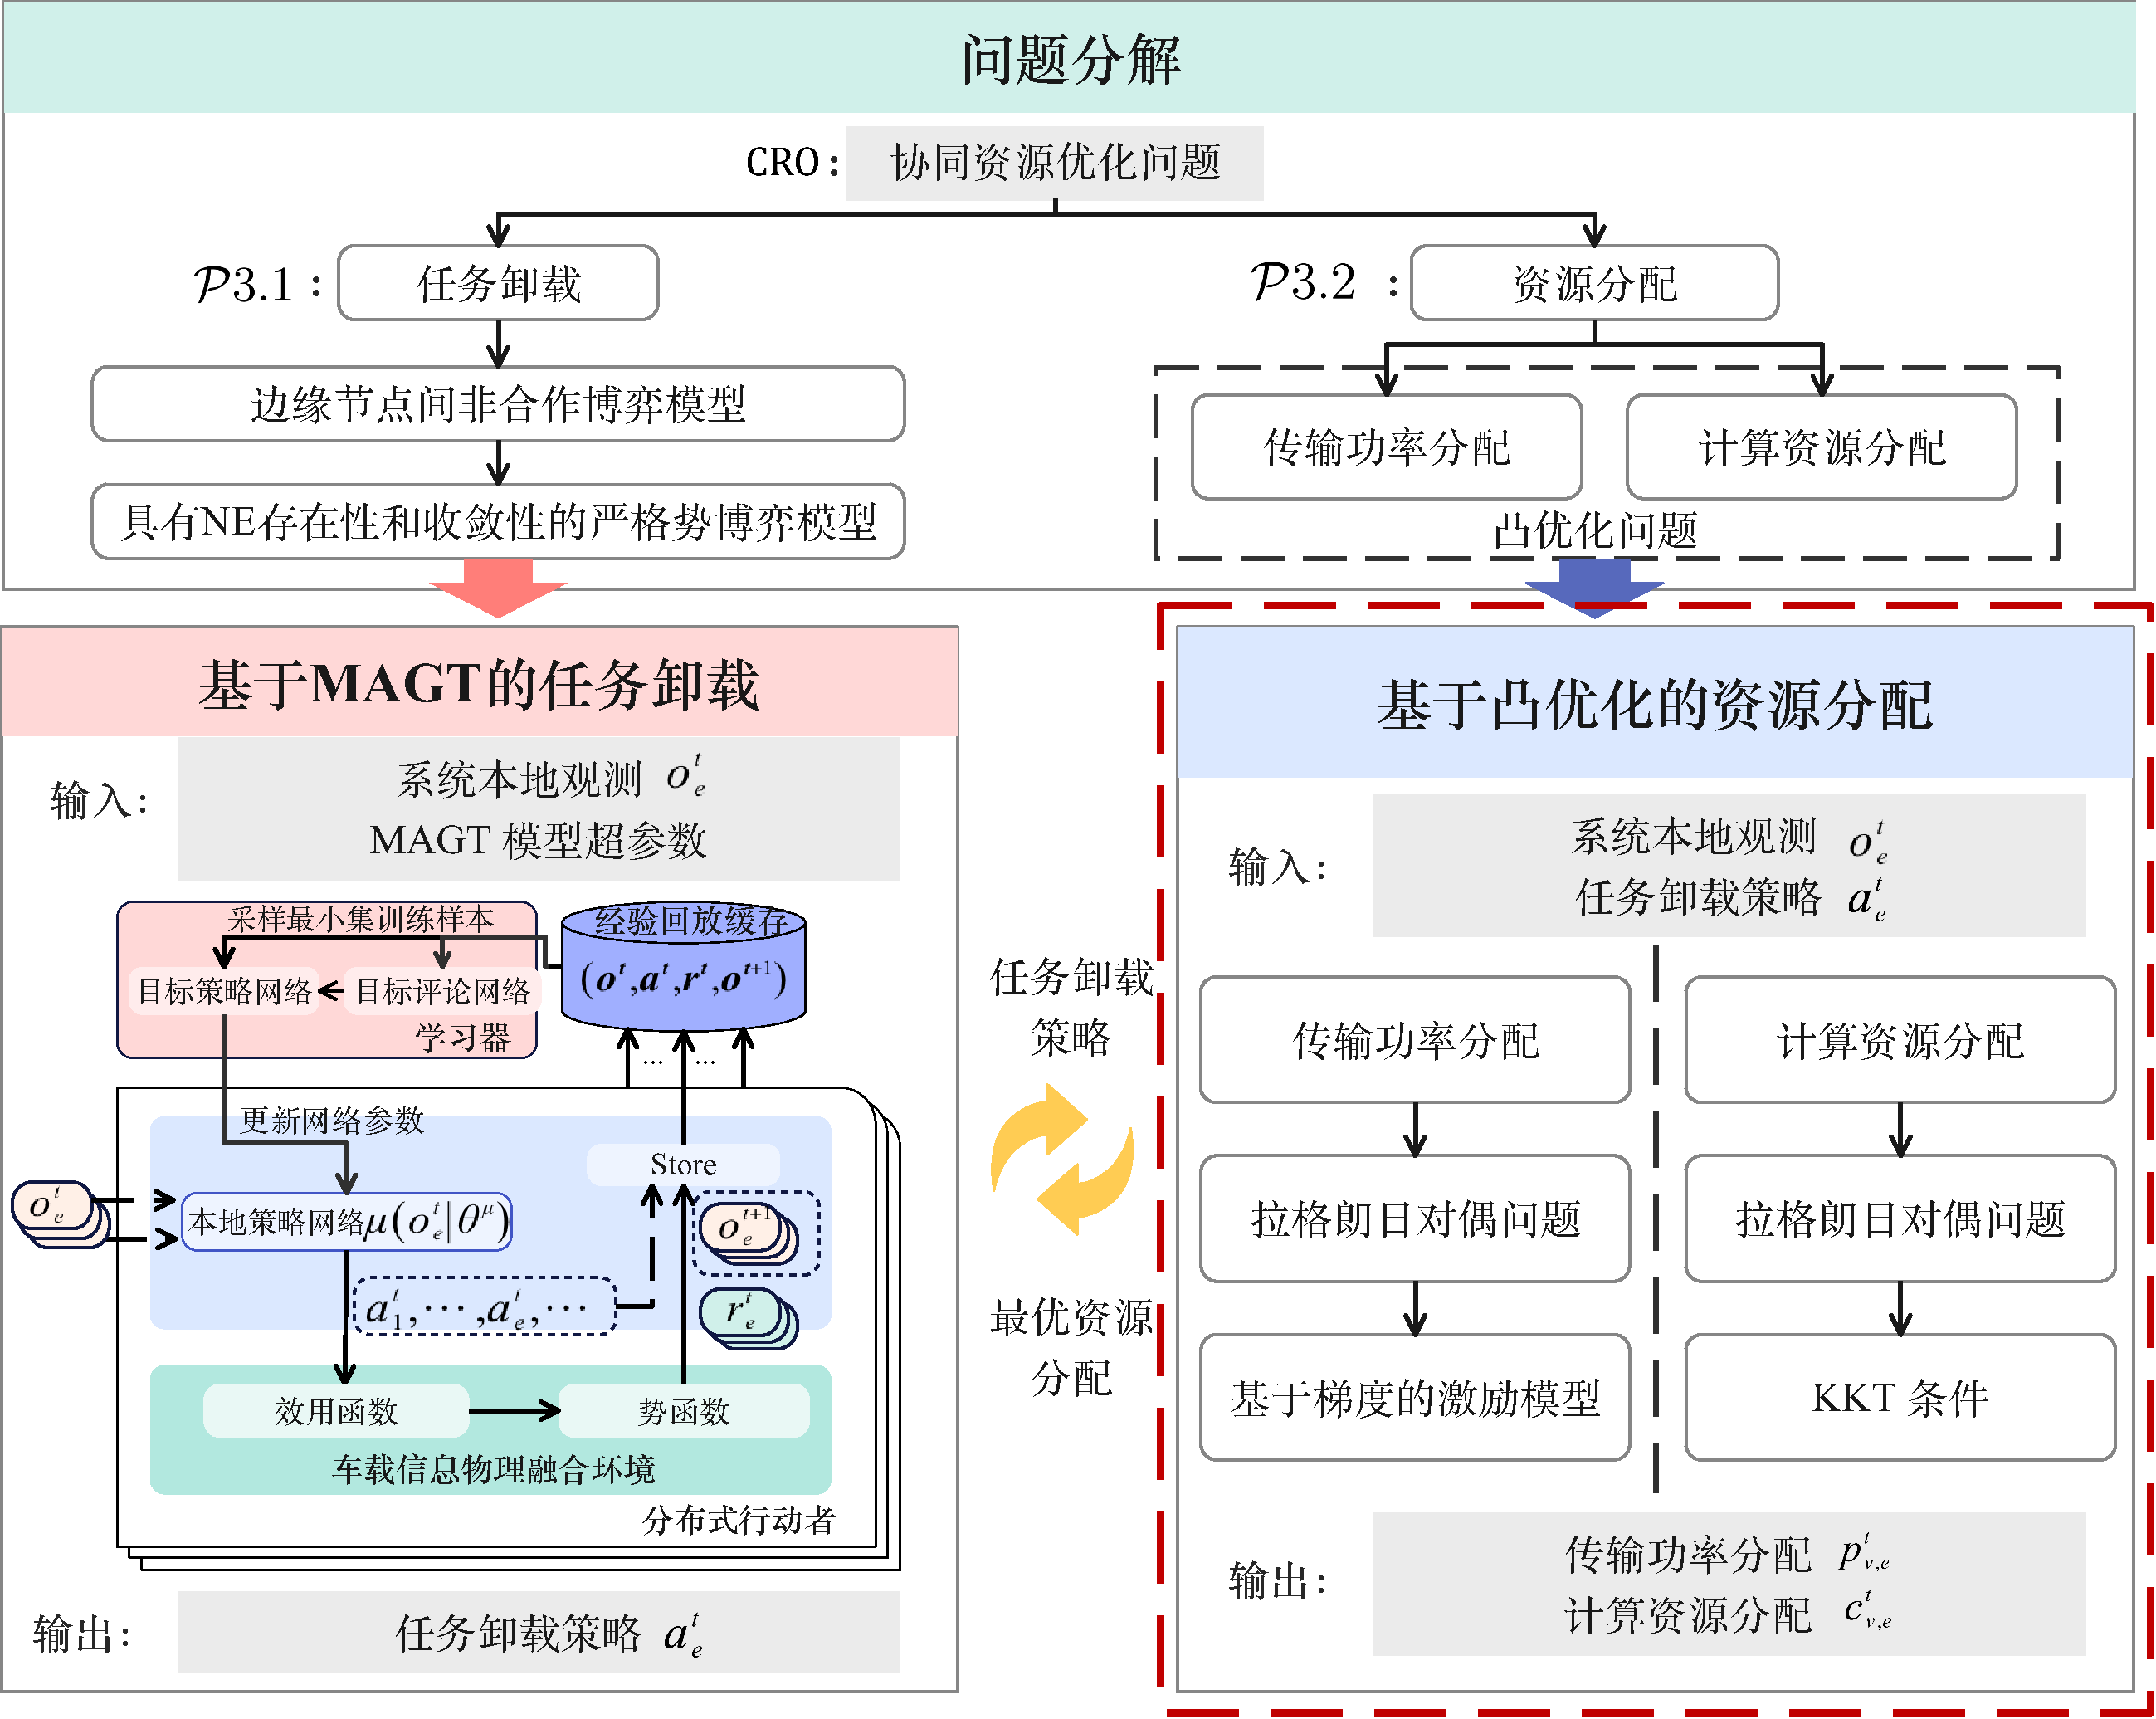
\includegraphics[width=0.45\textwidth]{fig/Fig3-3-solution-model3.pdf}
\end{figure}
\end{textblock*}
\end{center}

\begin{center}
\begin{textblock*}{0.62\textwidth}(0.5cm,2cm)
\begin{itemize}[itemsep=0.2\baselineskip]  \englishfont
	\item[\ding{111}] {\color{cqublue}{传输功率分配}}
	\begin{itemize}[itemsep=0.2\baselineskip] 
	\begin{small}	
	\item[\ding{226}] 引入拉格朗日乘子
	\item $\mathcal{L}(\widetilde{\mathbf{{P}}_{e}^{t}}, {\lambda}_{e}^{t} ) = \widetilde{g_3^{e}} -  {\lambda}_{e}^{t} (\sum_{\forall v \in \mathbf{V}_{e}^{t}} 2^{\widetilde{p_{v, e}^{t}}} - p_{e} )$ 
	\item[\ding{226}] 对偶问题分解为{\color{cqublue}{两层优化问题}}
	\item[\ding{226}] \underline{外层}:固定$\widetilde{\mathbf{{P}}_{e}^{t}}$,优化${\lambda}_{e}^{t}$,梯度下降迭代更新
	\item[\ding{226}] \underline{内层}:固定${\lambda}_{e}^{t}$,优化$\widetilde{\mathbf{{P}}_{e}^{t}}$,寻找拉格朗日静止点
	\end{small}
	\end{itemize}
	\item[\ding{111}] {\color{cqublue}{计算资源分配}}
	\begin{itemize}[itemsep=0.2\baselineskip]  \small
			\item[\ding{226}] 基于KKT条件得到最优解
			\item ${c_{v, e}^{t}}^{\star} = \frac{1 / c_e \sqrt{d_k  c_k} } {\sum_{\forall k_{v}^{t} \in {\mathbf{K}_{q_e}^{t} }} 1 / c_e \sqrt{d_k  c_k}} , \forall k_{v}^{t} \in {\mathbf{K}_{q_e}^{t} } $
			\item 
		\end{itemize}
\end{itemize}
\end{textblock*}
\end{center}
\end{frame}

\begin{frame}
\frametitle{\englishfont \underline{实验}:数据与基本设置}
\newBackground
\begin{center}
	\begin{textblock*}{\textwidth}(-3.2cm,2.7cm)
	\begin{table}[h] \englishfont
\resizebox{0.5\textwidth}{!}{%
\begin{tabular}{cc}
\toprule 
\textbf{参数} & \textbf{值}         \\ \midrule
边缘节点计算能力      & {[}3, 10{]} GHz \\
请求任务大小        & {[}0.01, 5{]} MB               \\
有线传输速率       & 50 Mbps           \\
处理1 bit所需计算资源          & 500 cycles/bit              \\
V2I 带宽& 20 MHz\\
最大传输功率& 1$\times 10^3$ mW\\
策略网络         & 5 层全连接 (隐藏层 256-256-256)  \\
评论家网络         & 5 层全连接 (隐藏层 512-512-256) \\
学习率         & 1$\times10^{-4}$              \\
折扣因子        & 0.996              \\
经验回放缓存大小    & 1$\times10^{6}$          \\
批大小         & 256                \\ \bottomrule
\end{tabular}%
}
\end{table}
\end{textblock*}
\end{center}

\begin{center}
\begin{textblock*}{\textwidth}(0cm,1.8cm)
\begin{itemize} \englishfont 
	\item[\ding{111}] {\color{cqublue}{实验与模型参数}}
\end{itemize}
\end{textblock*}
\end{center}

\begin{center}
\begin{textblock*}{0.65\textwidth}(7.5cm,1.8cm)
\begin{itemize}[itemsep=0.2\baselineskip]  \englishfont 
	\item[\ding{111}] {\color{cqublue}{对比算法}}
	\begin{itemize}[itemsep=0.2\baselineskip] 
	\begin{small}
		\item[\ding{226}] 最优资源分配和任务全迁移 ({\color{red}{ORM}})
		\item[\ding{226}] 最优资源分配和任务仅本地处理 ({\color{red}{ORL}})
		\item[\ding{226}] 分布式深度确定性策略梯度 ({\color{red}{D4PG}})
		\item[\ding{226}] 多智能体深度确定性策略梯度 ({\color{red}{MADDPG}})
		\item
	\end{small}
	\end{itemize}
\end{itemize}
\end{textblock*}
\end{center}

\begin{center}
\begin{textblock*}{0.55\textwidth}(7.5cm,4.5cm)
\begin{itemize}[itemsep=0.2\baselineskip] \englishfont
	\item[\ding{111}] {\color{cqublue}{性能评估指标}}
	\begin{itemize}[itemsep=0.2\baselineskip]
	\begin{small}
		\item[\ding{226}] 累计奖励 ({\color{red}{CR}})
		\item[\ding{226}] 平均服务率 ({\color{red}{ASR}})
		\item[\ding{226}] 平均实现势 ({\color{red}{AAP}})\\
			{\small{$\operatorname{AAP} = \frac{1}{E}\sum_{\forall e \in \mathbf{E}} \sum_{\forall t \in \mathbf{T}} r_{e}^{t}$}}
		\item[\ding{226}] 本地处理与迁移的比例 ({\color{red}{PLPM}})\\
{\small{$P_{\operatorname{local}} = \frac{K_{\operatorname{local}}}{K_{\operatorname{total}}}$}} \hspace{1em}{\small{$P_{\operatorname{migrated}} = \frac{K_{\operatorname{migrated}}}{K_{\operatorname{total}}}$}}
	\end{small}
	\end{itemize}
\end{itemize}
\end{textblock*}
\end{center}

\end{frame}

\begin{frame}
\newBackground

\begin{overlayarea}{\textwidth}{3cm}
\only<1-1>{
\frametitle{\englishfont \underline{实验}:算法收敛性}
\begin{center} \englishfont \footnotesize
\begin{textblock*}{\textwidth}(1cm,1.8cm)
	\begin{figure}
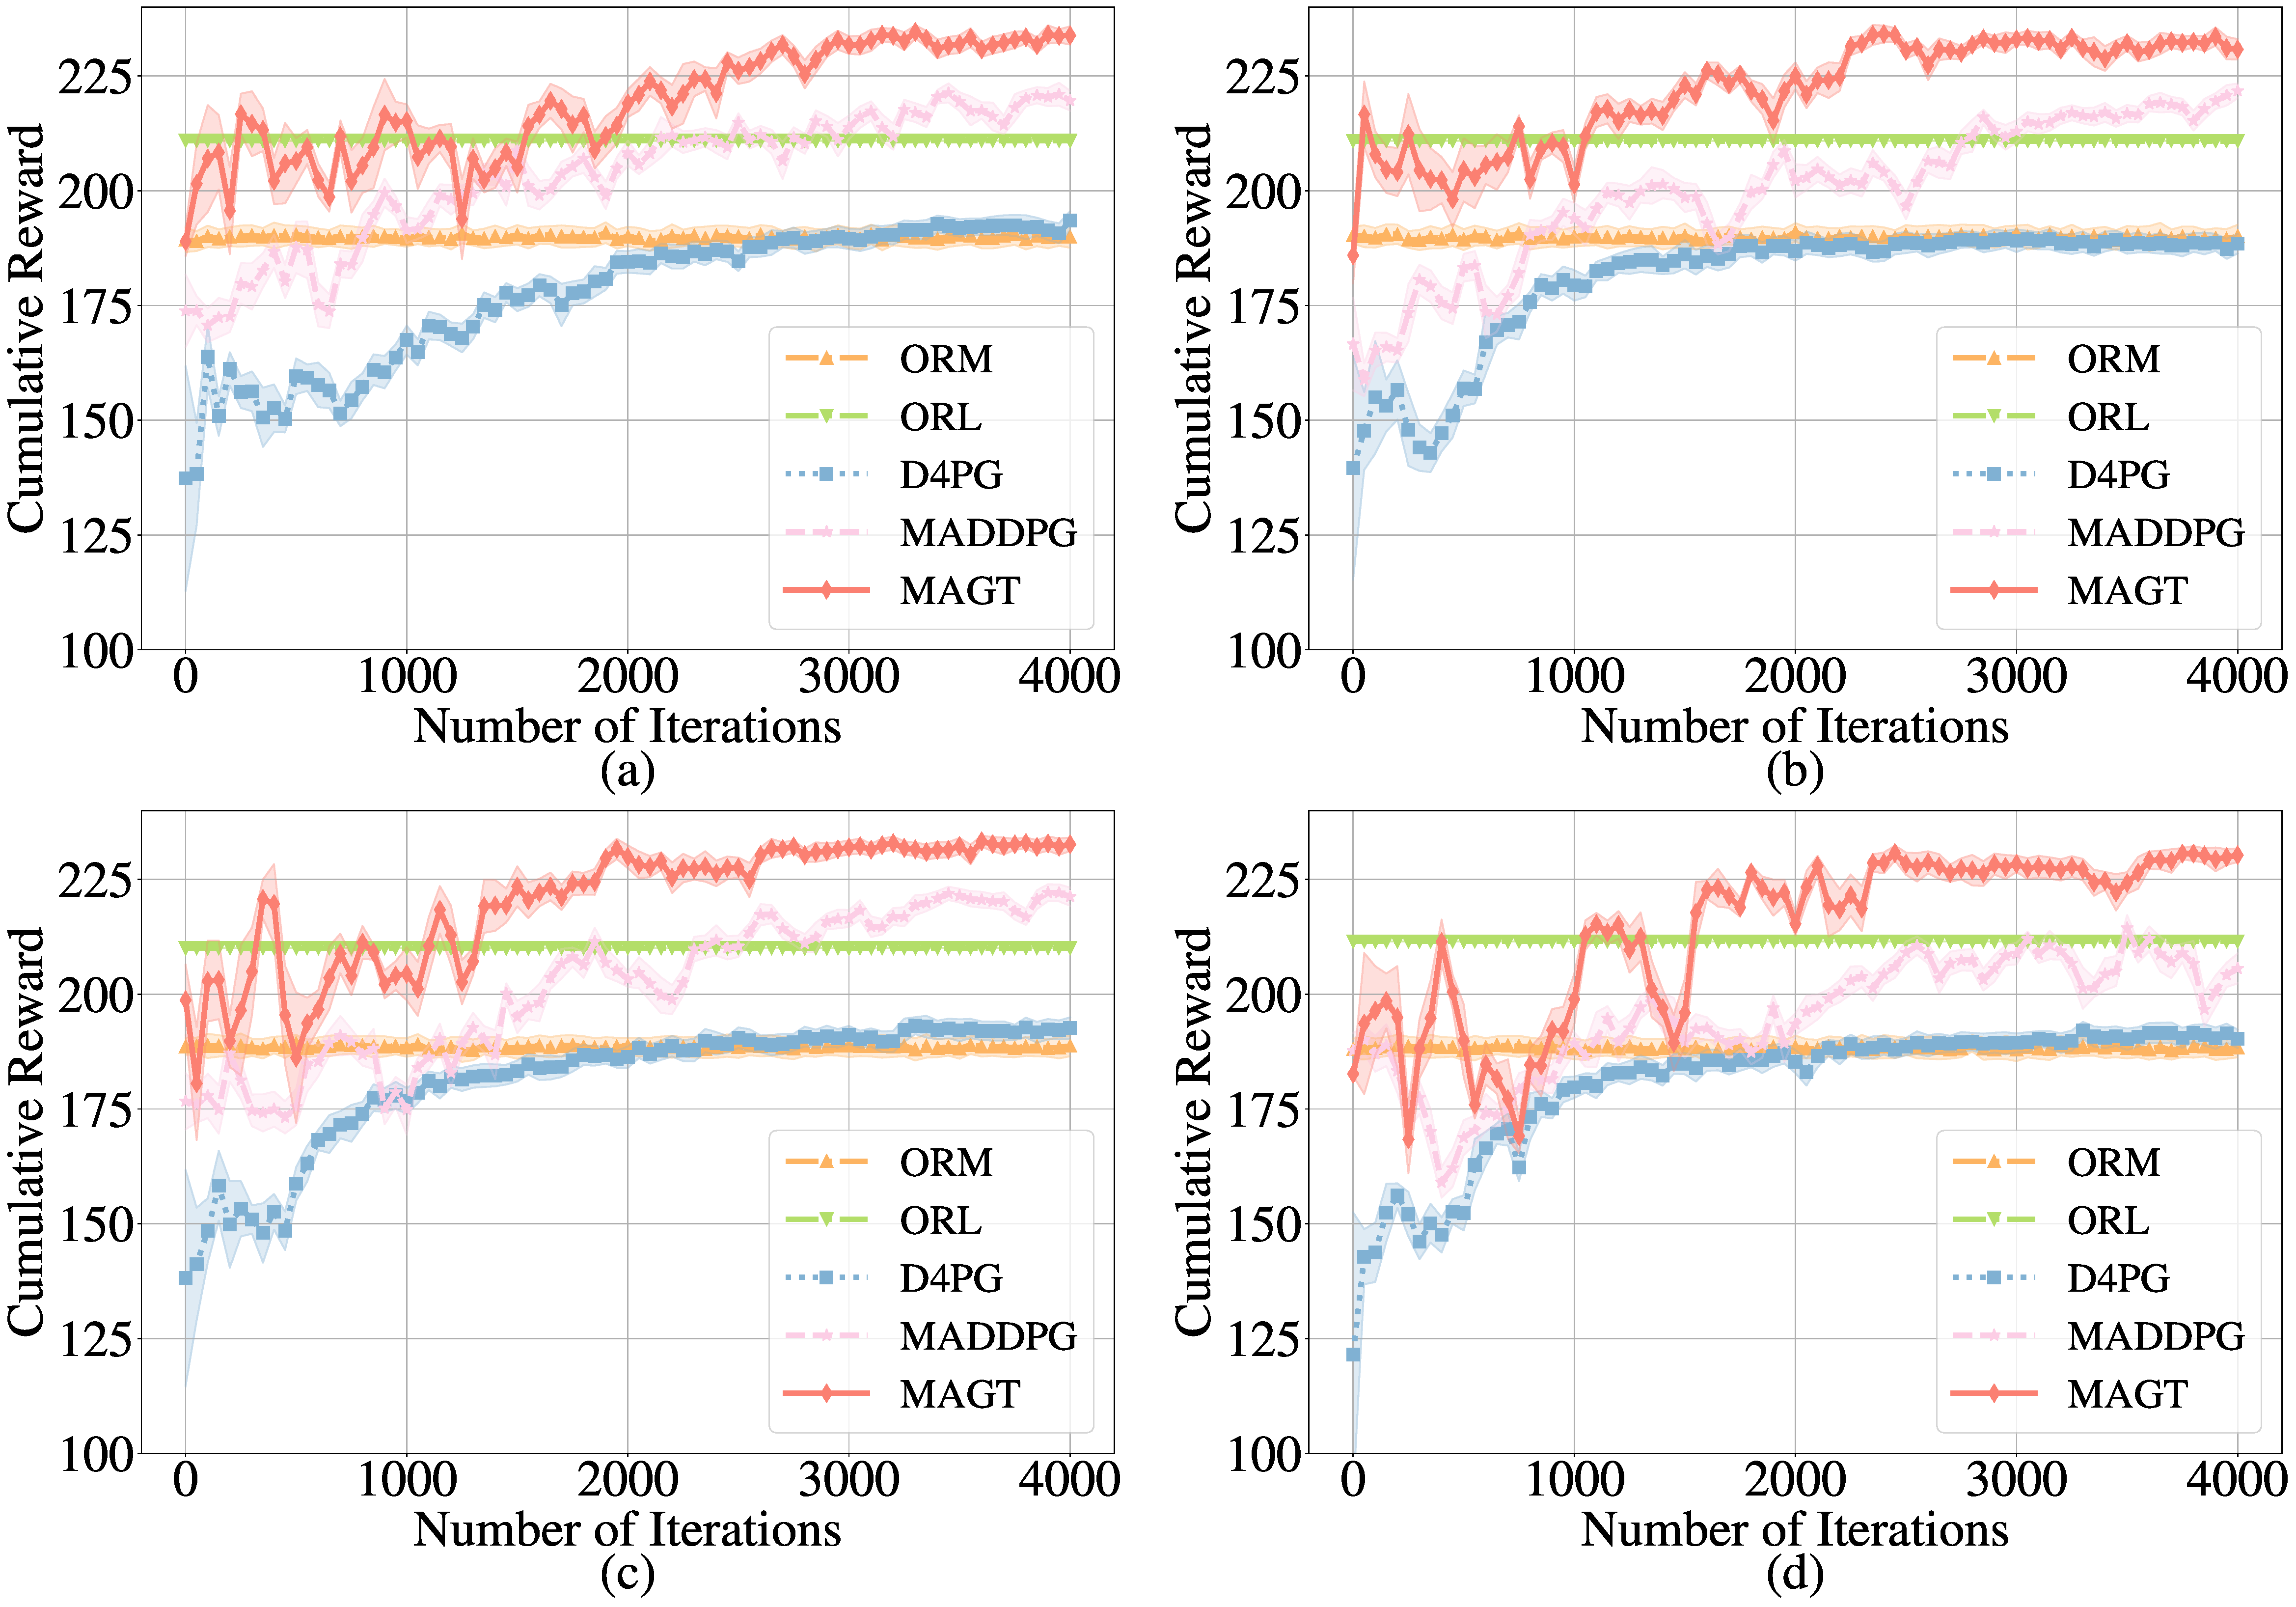
\includegraphics[width=0.65\textwidth]{fig/Fig3-4-convergence.pdf}
	\end{figure}
\end{textblock*}
\end{center}
}

\only<2-2>{
\frametitle{\englishfont \underline{实验}:算法收敛性}
\begin{center} \englishfont \footnotesize
\begin{textblock*}{\textwidth}(1cm,1.8cm)
	\begin{figure}
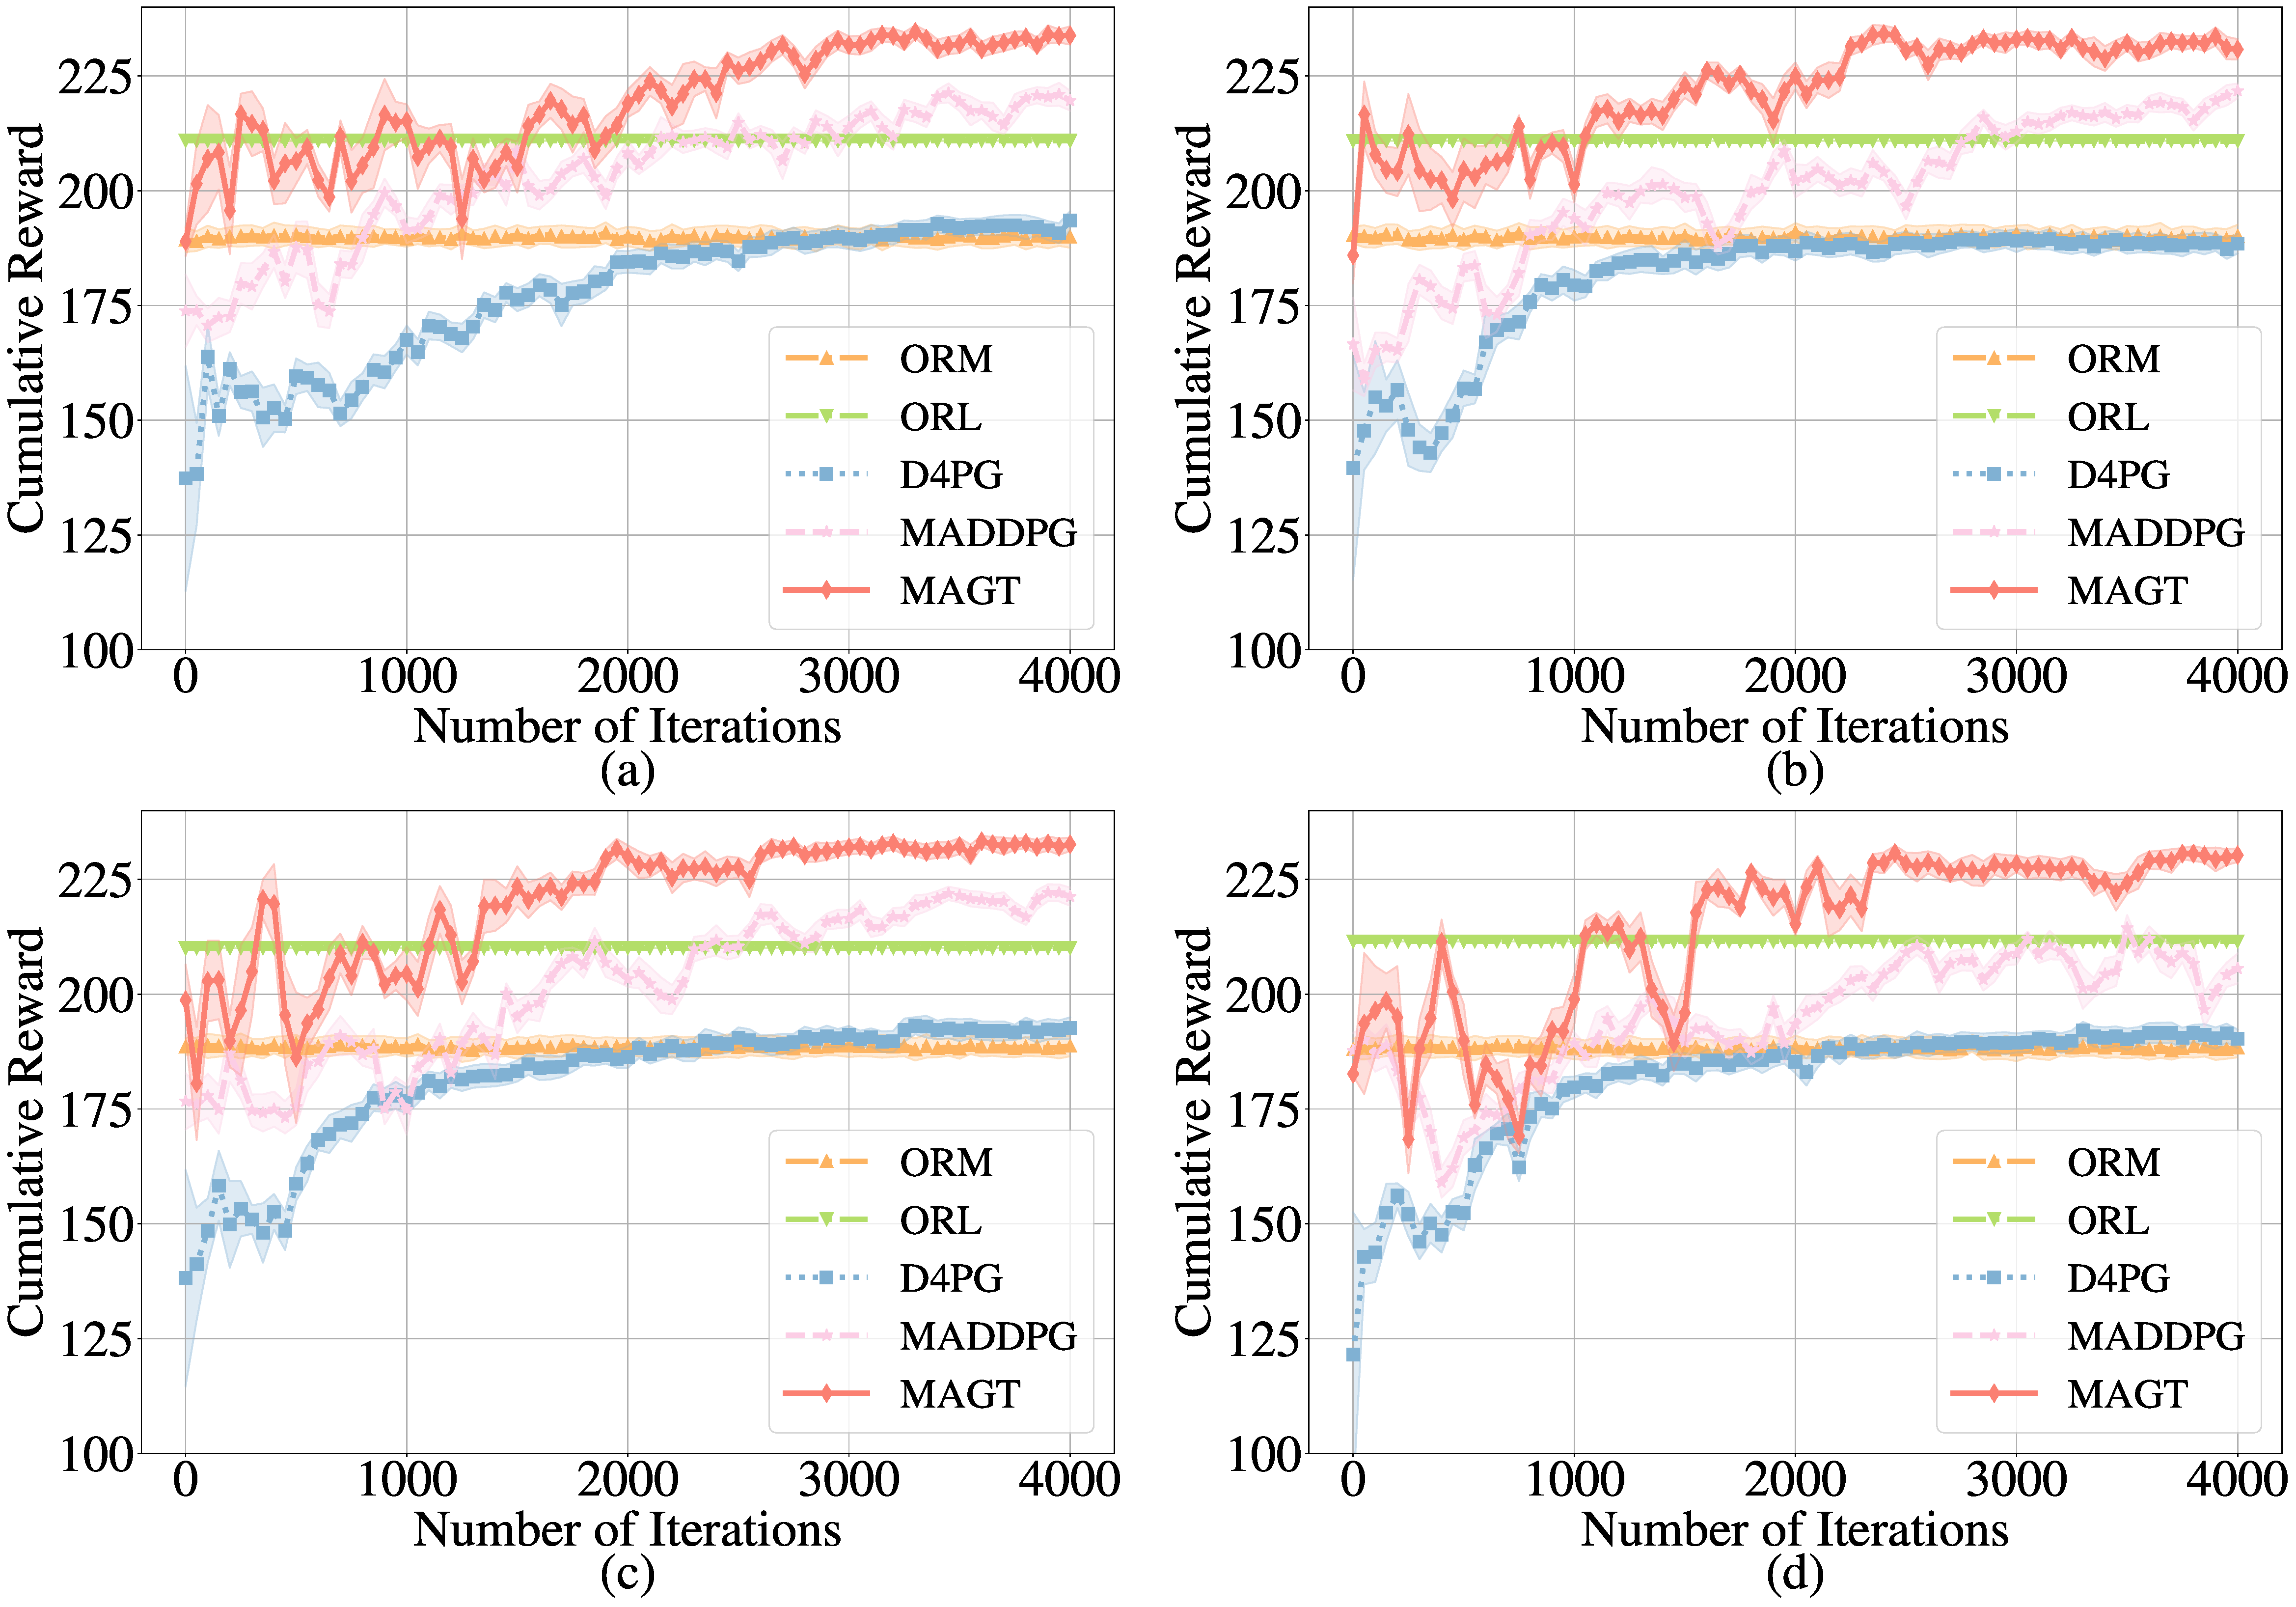
\includegraphics[width=0.65\textwidth]{fig/Fig3-4-convergence.pdf}
	\end{figure}
\end{textblock*}
\end{center}
}

\only<2-2>{
\begin{center} \englishfont \footnotesize
\begin{textblock*}{\textwidth}(0cm,1.6cm)
{\LARGE{\color{red}\ding{216}}}
\end{textblock*}
\end{center}

\begin{center} \englishfont \footnotesize
\begin{textblock*}{\textwidth}(5cm,1.6cm)
{\LARGE{\color{red}\ding{216}}}
\end{textblock*}
\end{center}

\begin{center} \englishfont \footnotesize
\begin{textblock*}{\textwidth}(0cm,4.8cm)
{\LARGE{\color{red}\ding{216}}}
\end{textblock*}
\end{center}

\begin{center} \englishfont \footnotesize
\begin{textblock*}{\textwidth}(5cm,4.8cm)
{\LARGE{\color{red}\ding{216}}}
\end{textblock*}
\end{center}
}

\only<3-3>{
\frametitle{\englishfont \underline{实验}:交通场景的影响}
\begin{center} \englishfont \footnotesize
\begin{textblock*}{\textwidth}(1cm,1.8cm)
	\begin{figure}
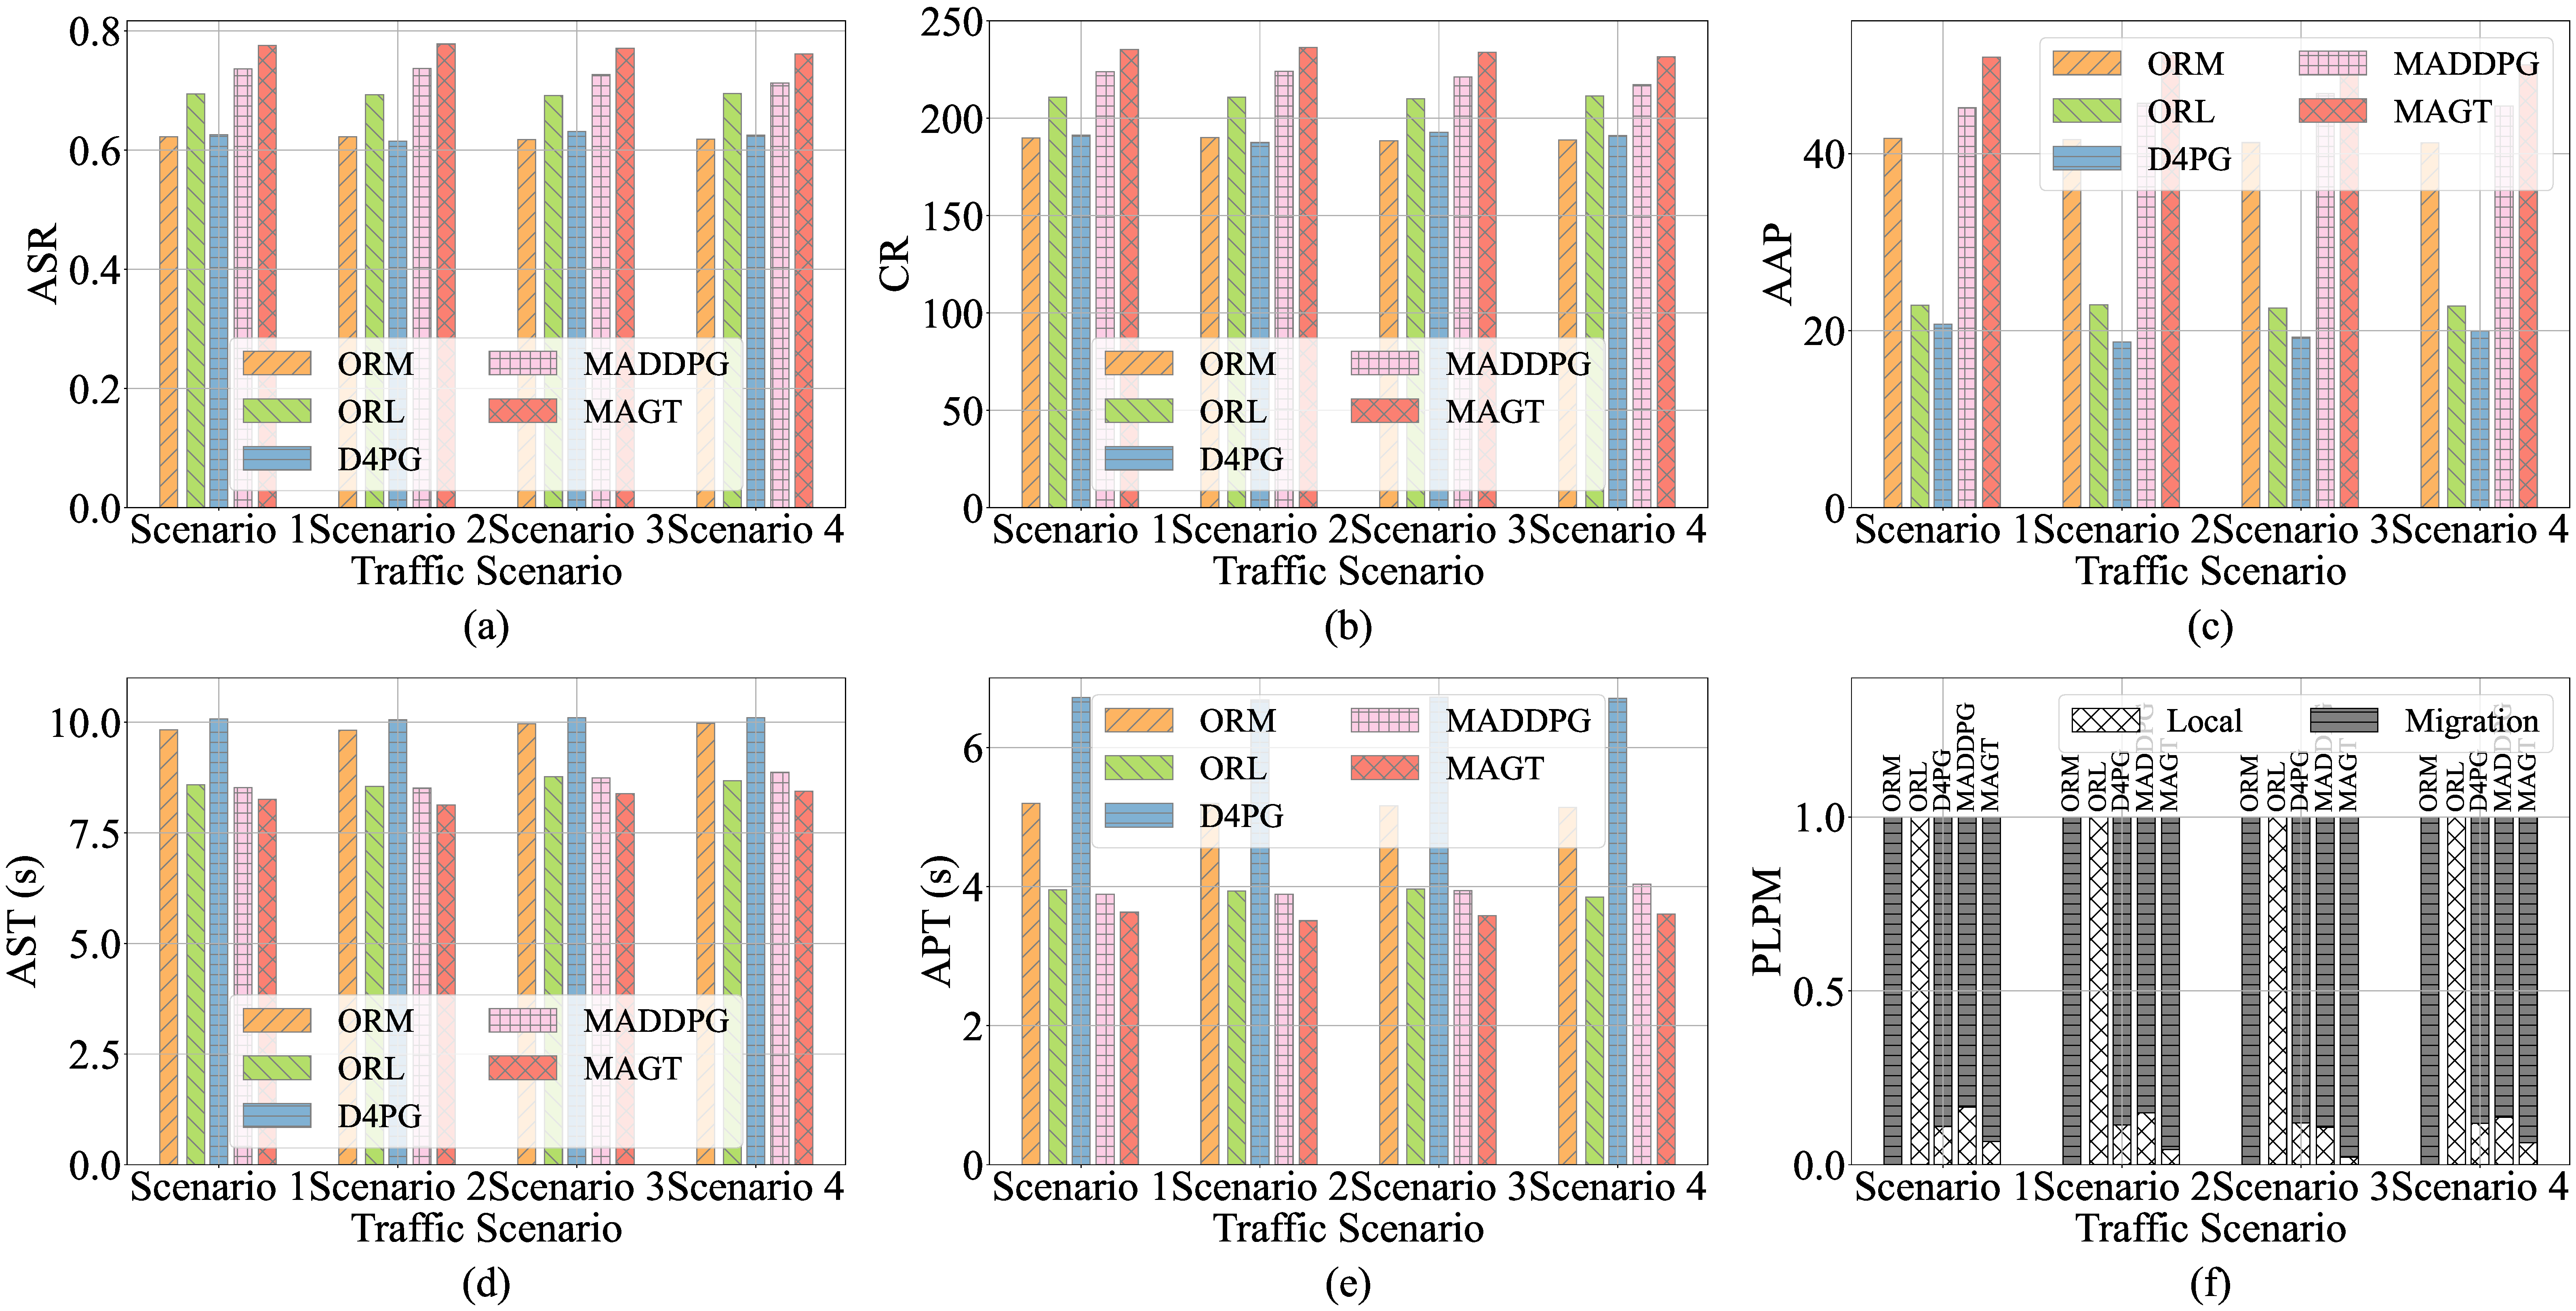
\includegraphics[width=0.9\textwidth]{fig/Fig3-5-different-traffica-scenarios.pdf}
	\end{figure}
\end{textblock*}
\end{center}
}

\only<4-4>{
\frametitle{\englishfont \underline{实验}:交通场景的影响}
\begin{center} \englishfont \footnotesize
\begin{textblock*}{\textwidth}(1cm,1.8cm)
	\begin{figure}
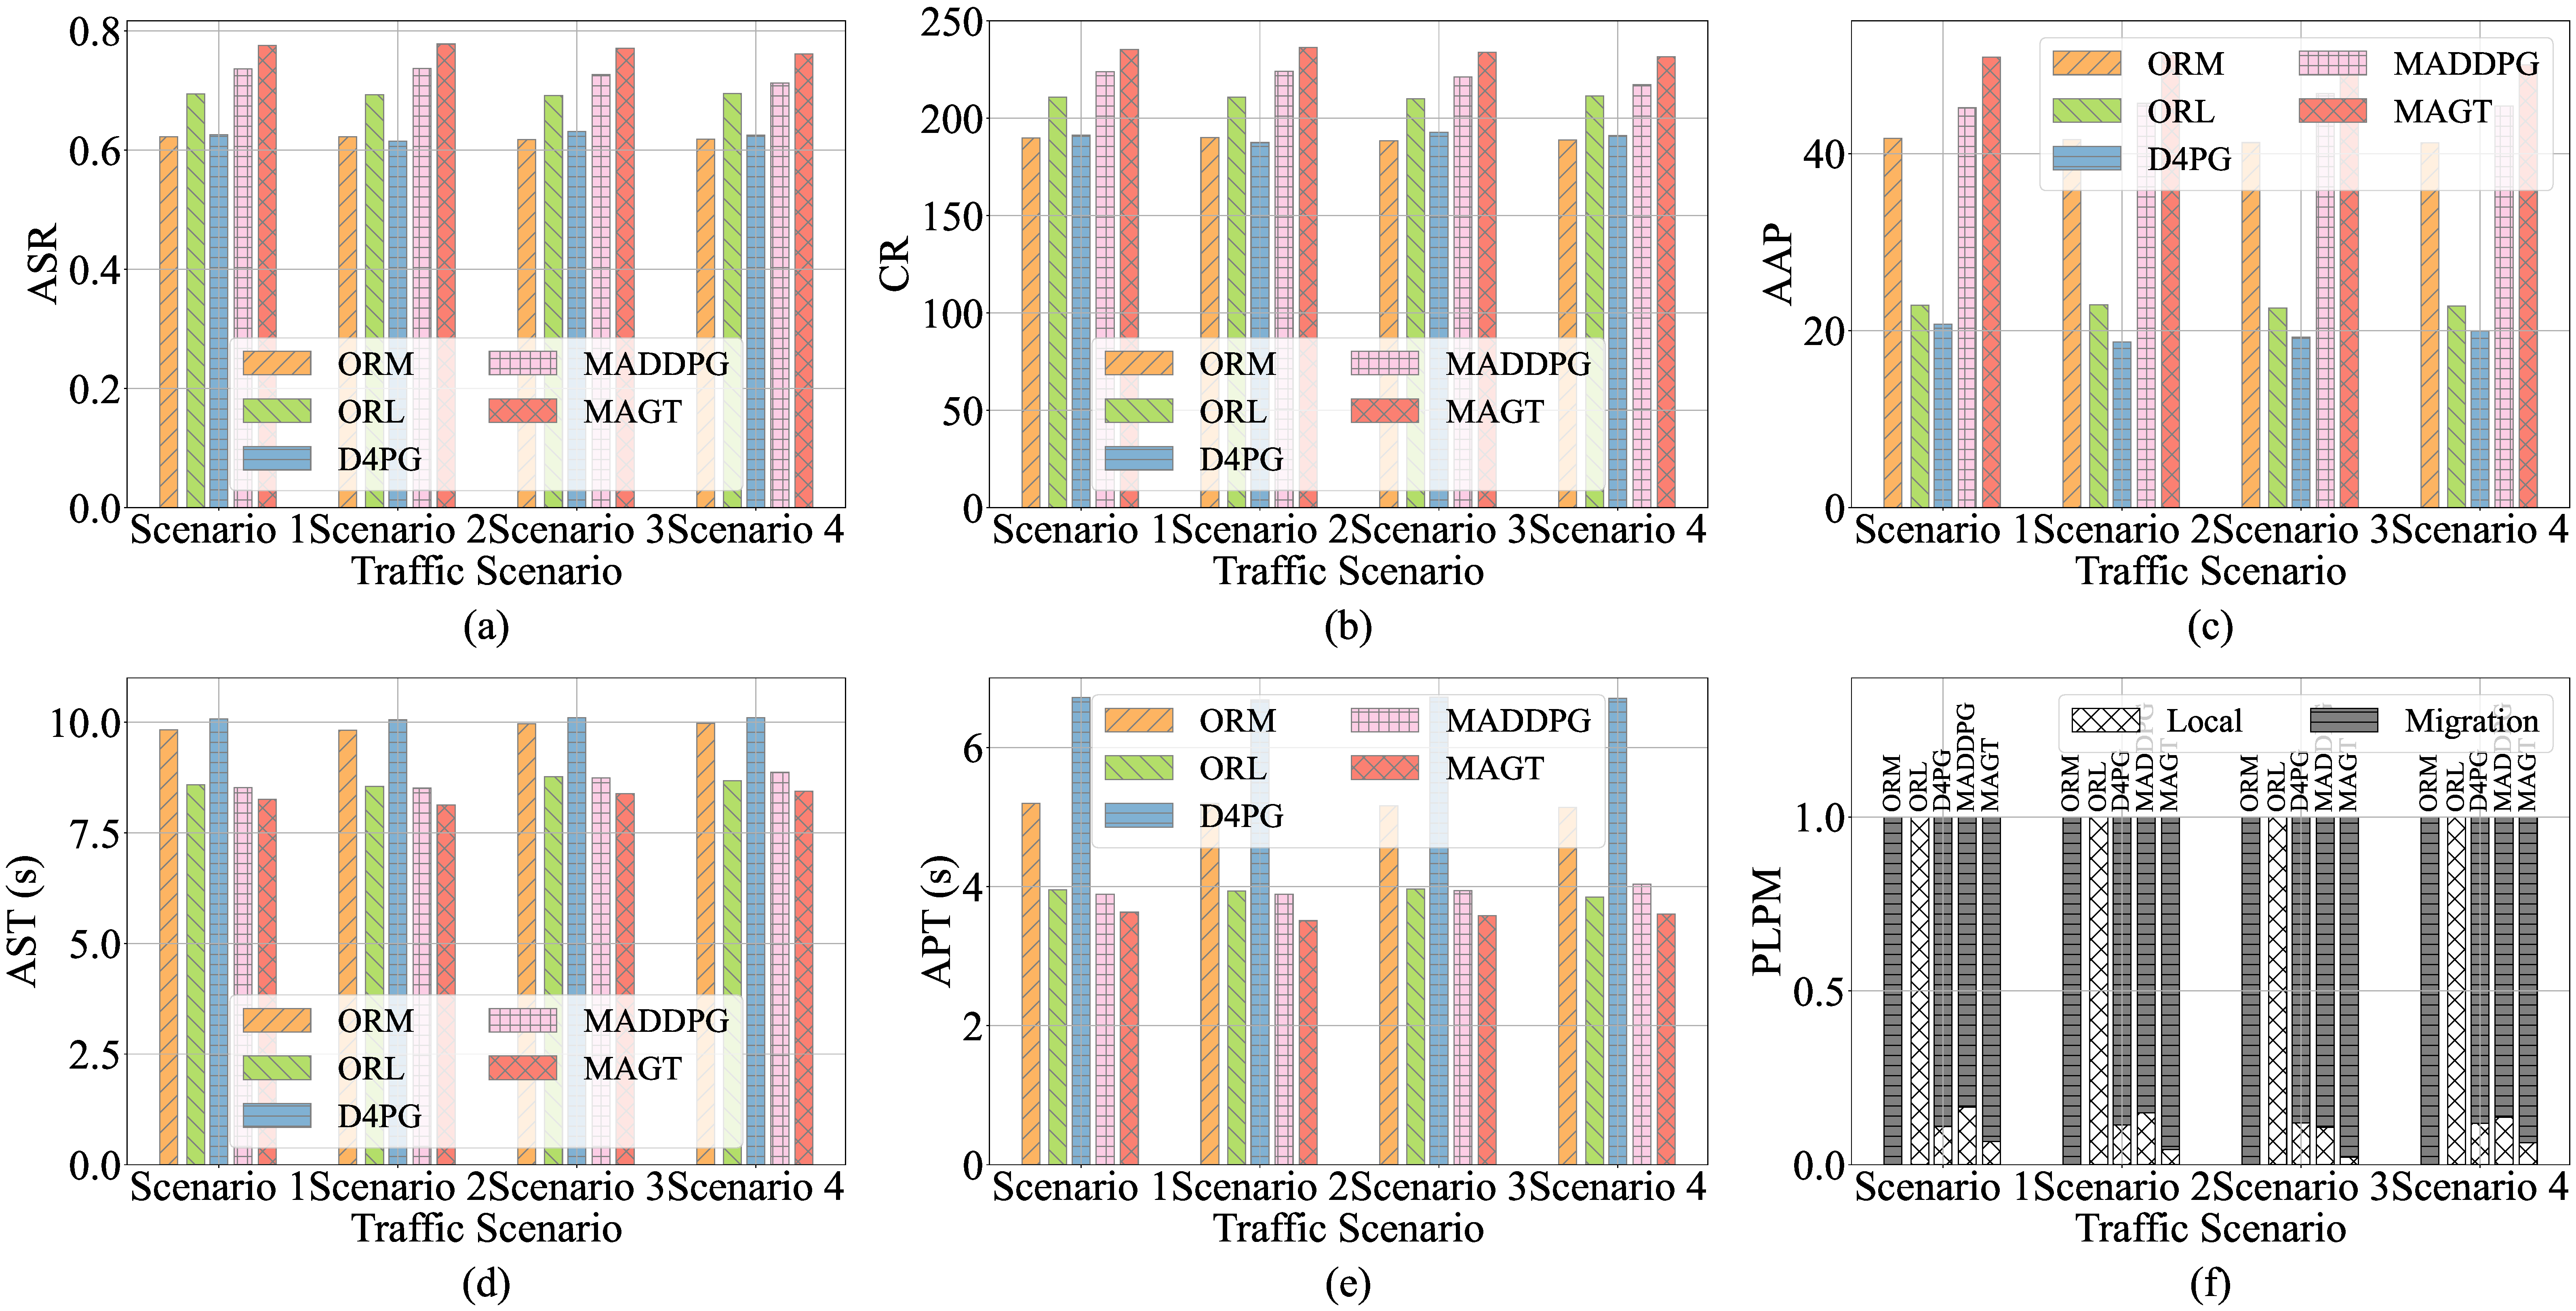
\includegraphics[width=0.9\textwidth]{fig/Fig3-5-different-traffica-scenarios.pdf}
	\end{figure}
\end{textblock*}
\end{center}
}

\only<4-4>{
\begin{center} \englishfont \footnotesize
\begin{textblock*}{\textwidth}(-3.3cm,1.65cm)
{\LARGE{\color{red}\ding{216}}}
\end{textblock*}
\end{center}

\begin{center} \englishfont \footnotesize
\begin{textblock*}{\textwidth}(0.9cm,1.7cm)
{\LARGE{\color{red}\ding{216}}}
\end{textblock*}
\end{center}

\begin{center} \englishfont \footnotesize
\begin{textblock*}{\textwidth}(4.25cm,1.75cm)
{\LARGE{\color{red}\ding{216}}}
\end{textblock*}
\end{center}

\begin{center} \englishfont \footnotesize
\begin{textblock*}{\textwidth}(0.9cm,5.95cm)
{\LARGE{\color{red}\ding{216}}}
\end{textblock*}
\end{center}

\begin{center} \englishfont \footnotesize
\begin{textblock*}{\textwidth}(-3.3cm,5.4cm)
{\LARGE{\color{red}\ding{216}}}
\end{textblock*}
\end{center}
}

\only<5-5>{
\frametitle{\englishfont \underline{实验}:计算能力的影响}
\begin{center} \englishfont \footnotesize
\begin{textblock*}{\textwidth}(1cm,1.8cm)
	\begin{figure}
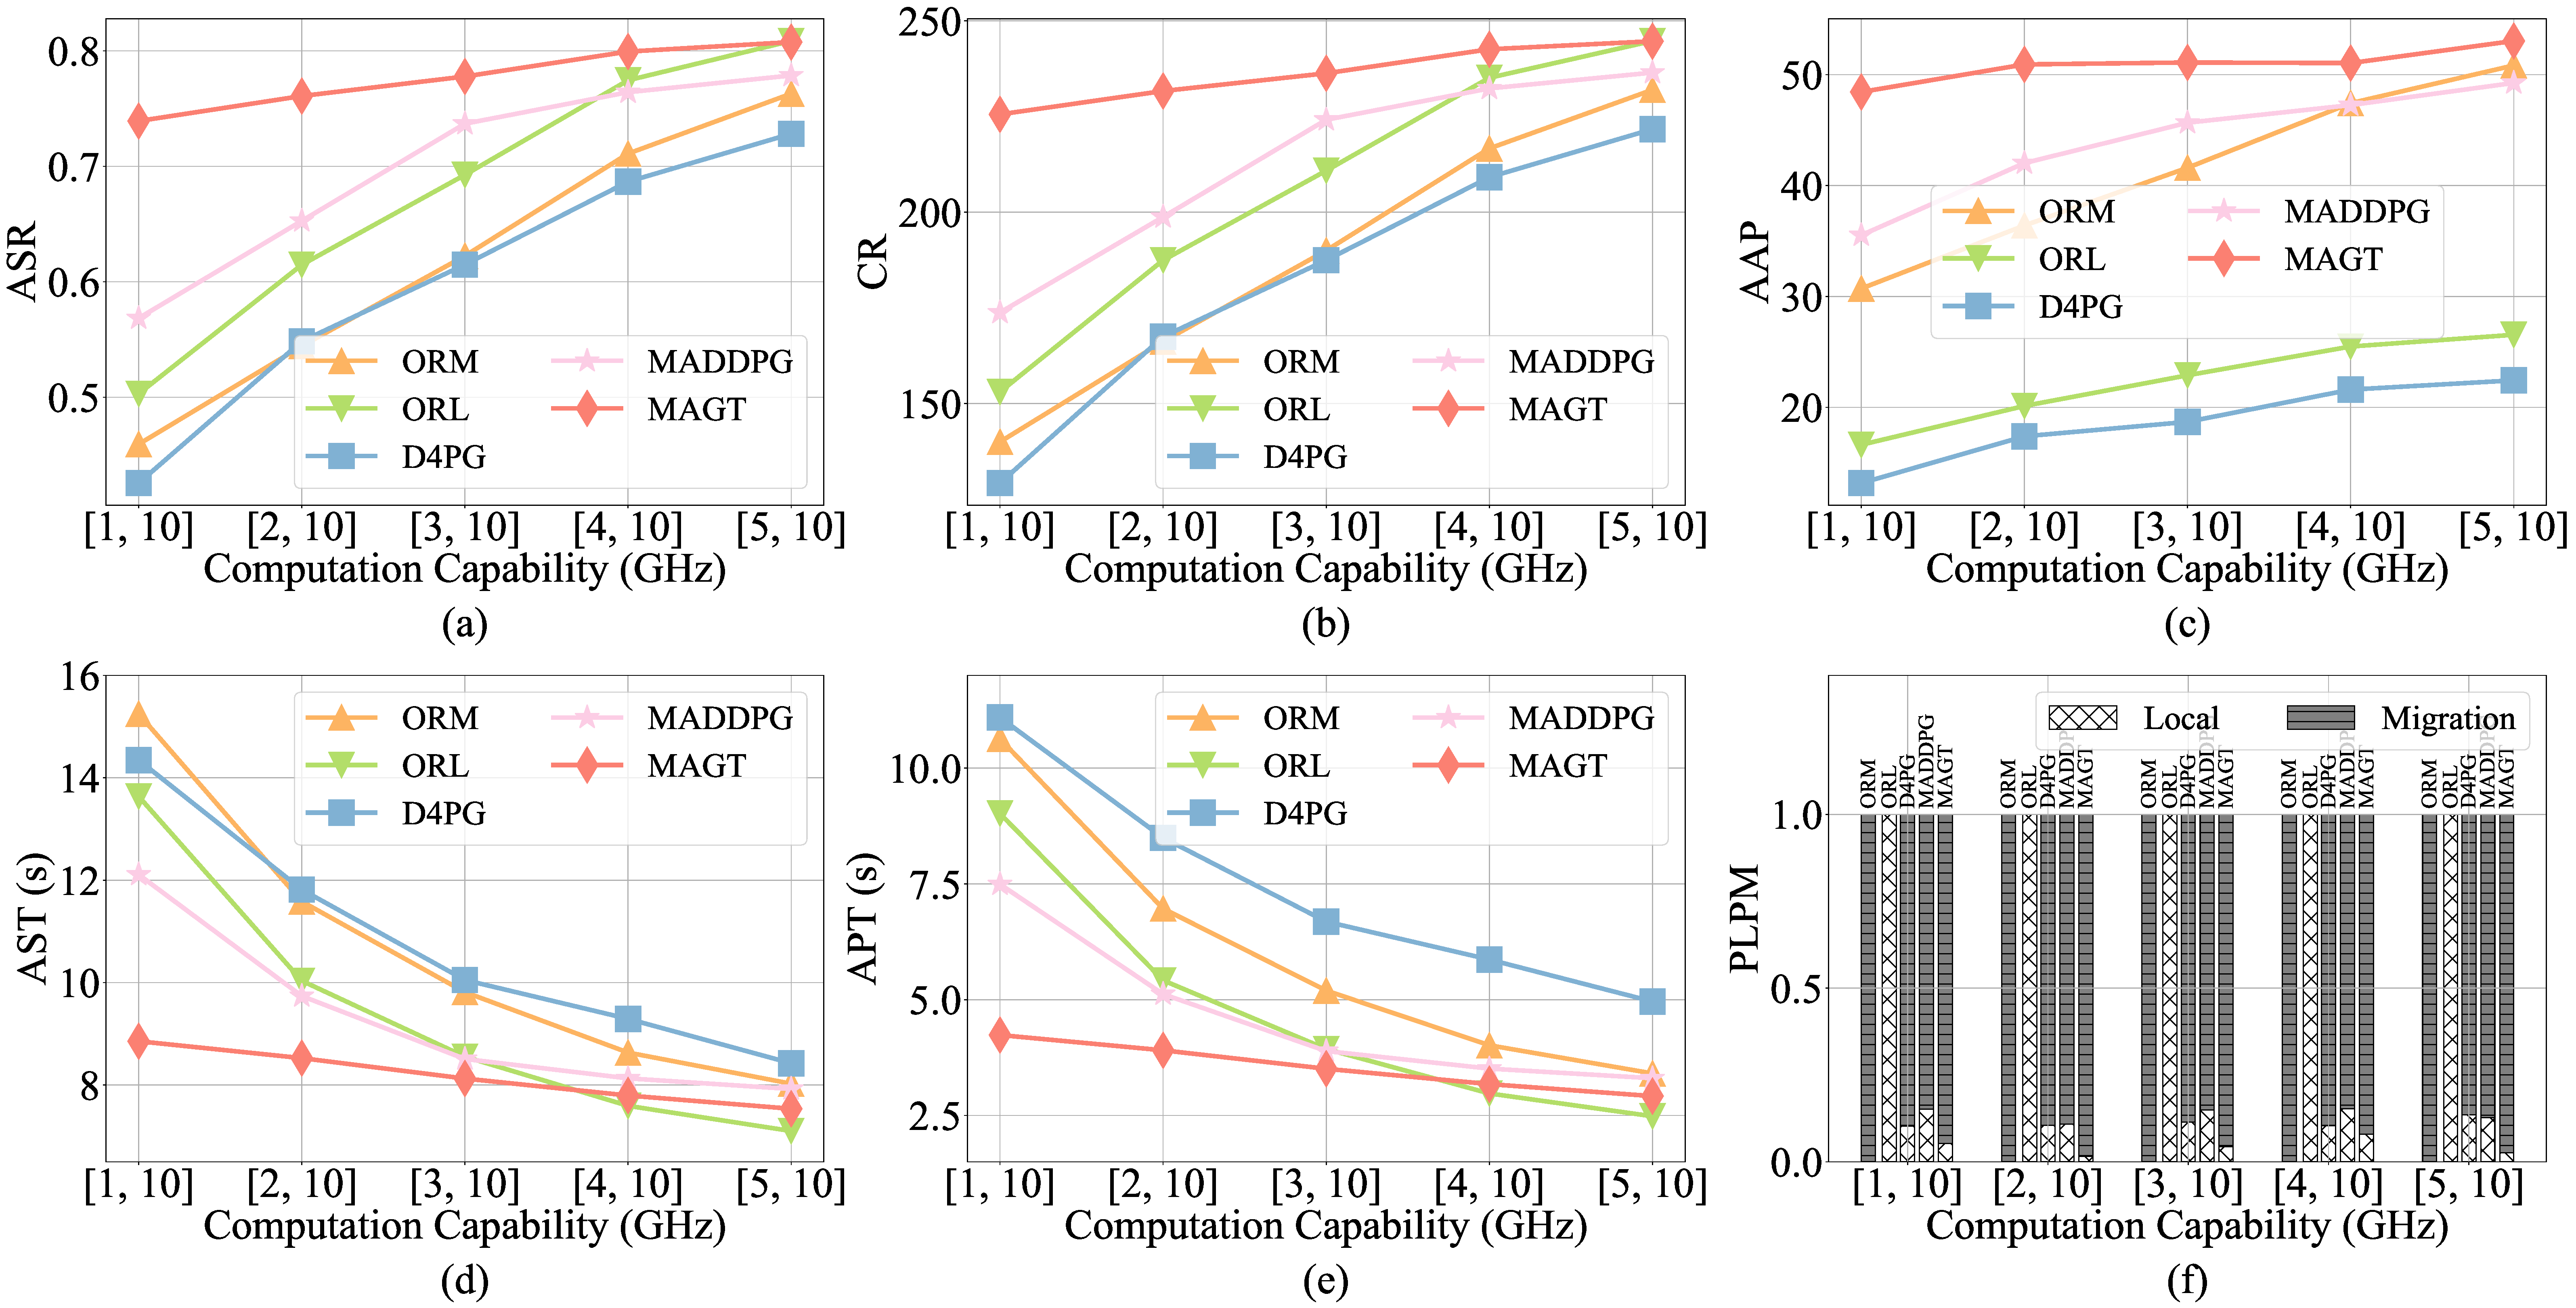
\includegraphics[width=0.9\textwidth]{fig/Fig3-6-different-computation-capability.pdf}
	\end{figure}
\end{textblock*}
\end{center}
}

\only<6-6>{
\frametitle{\englishfont \underline{实验}:计算能力的影响}
\begin{center} \englishfont \footnotesize
\begin{textblock*}{\textwidth}(1cm,1.8cm)
	\begin{figure}
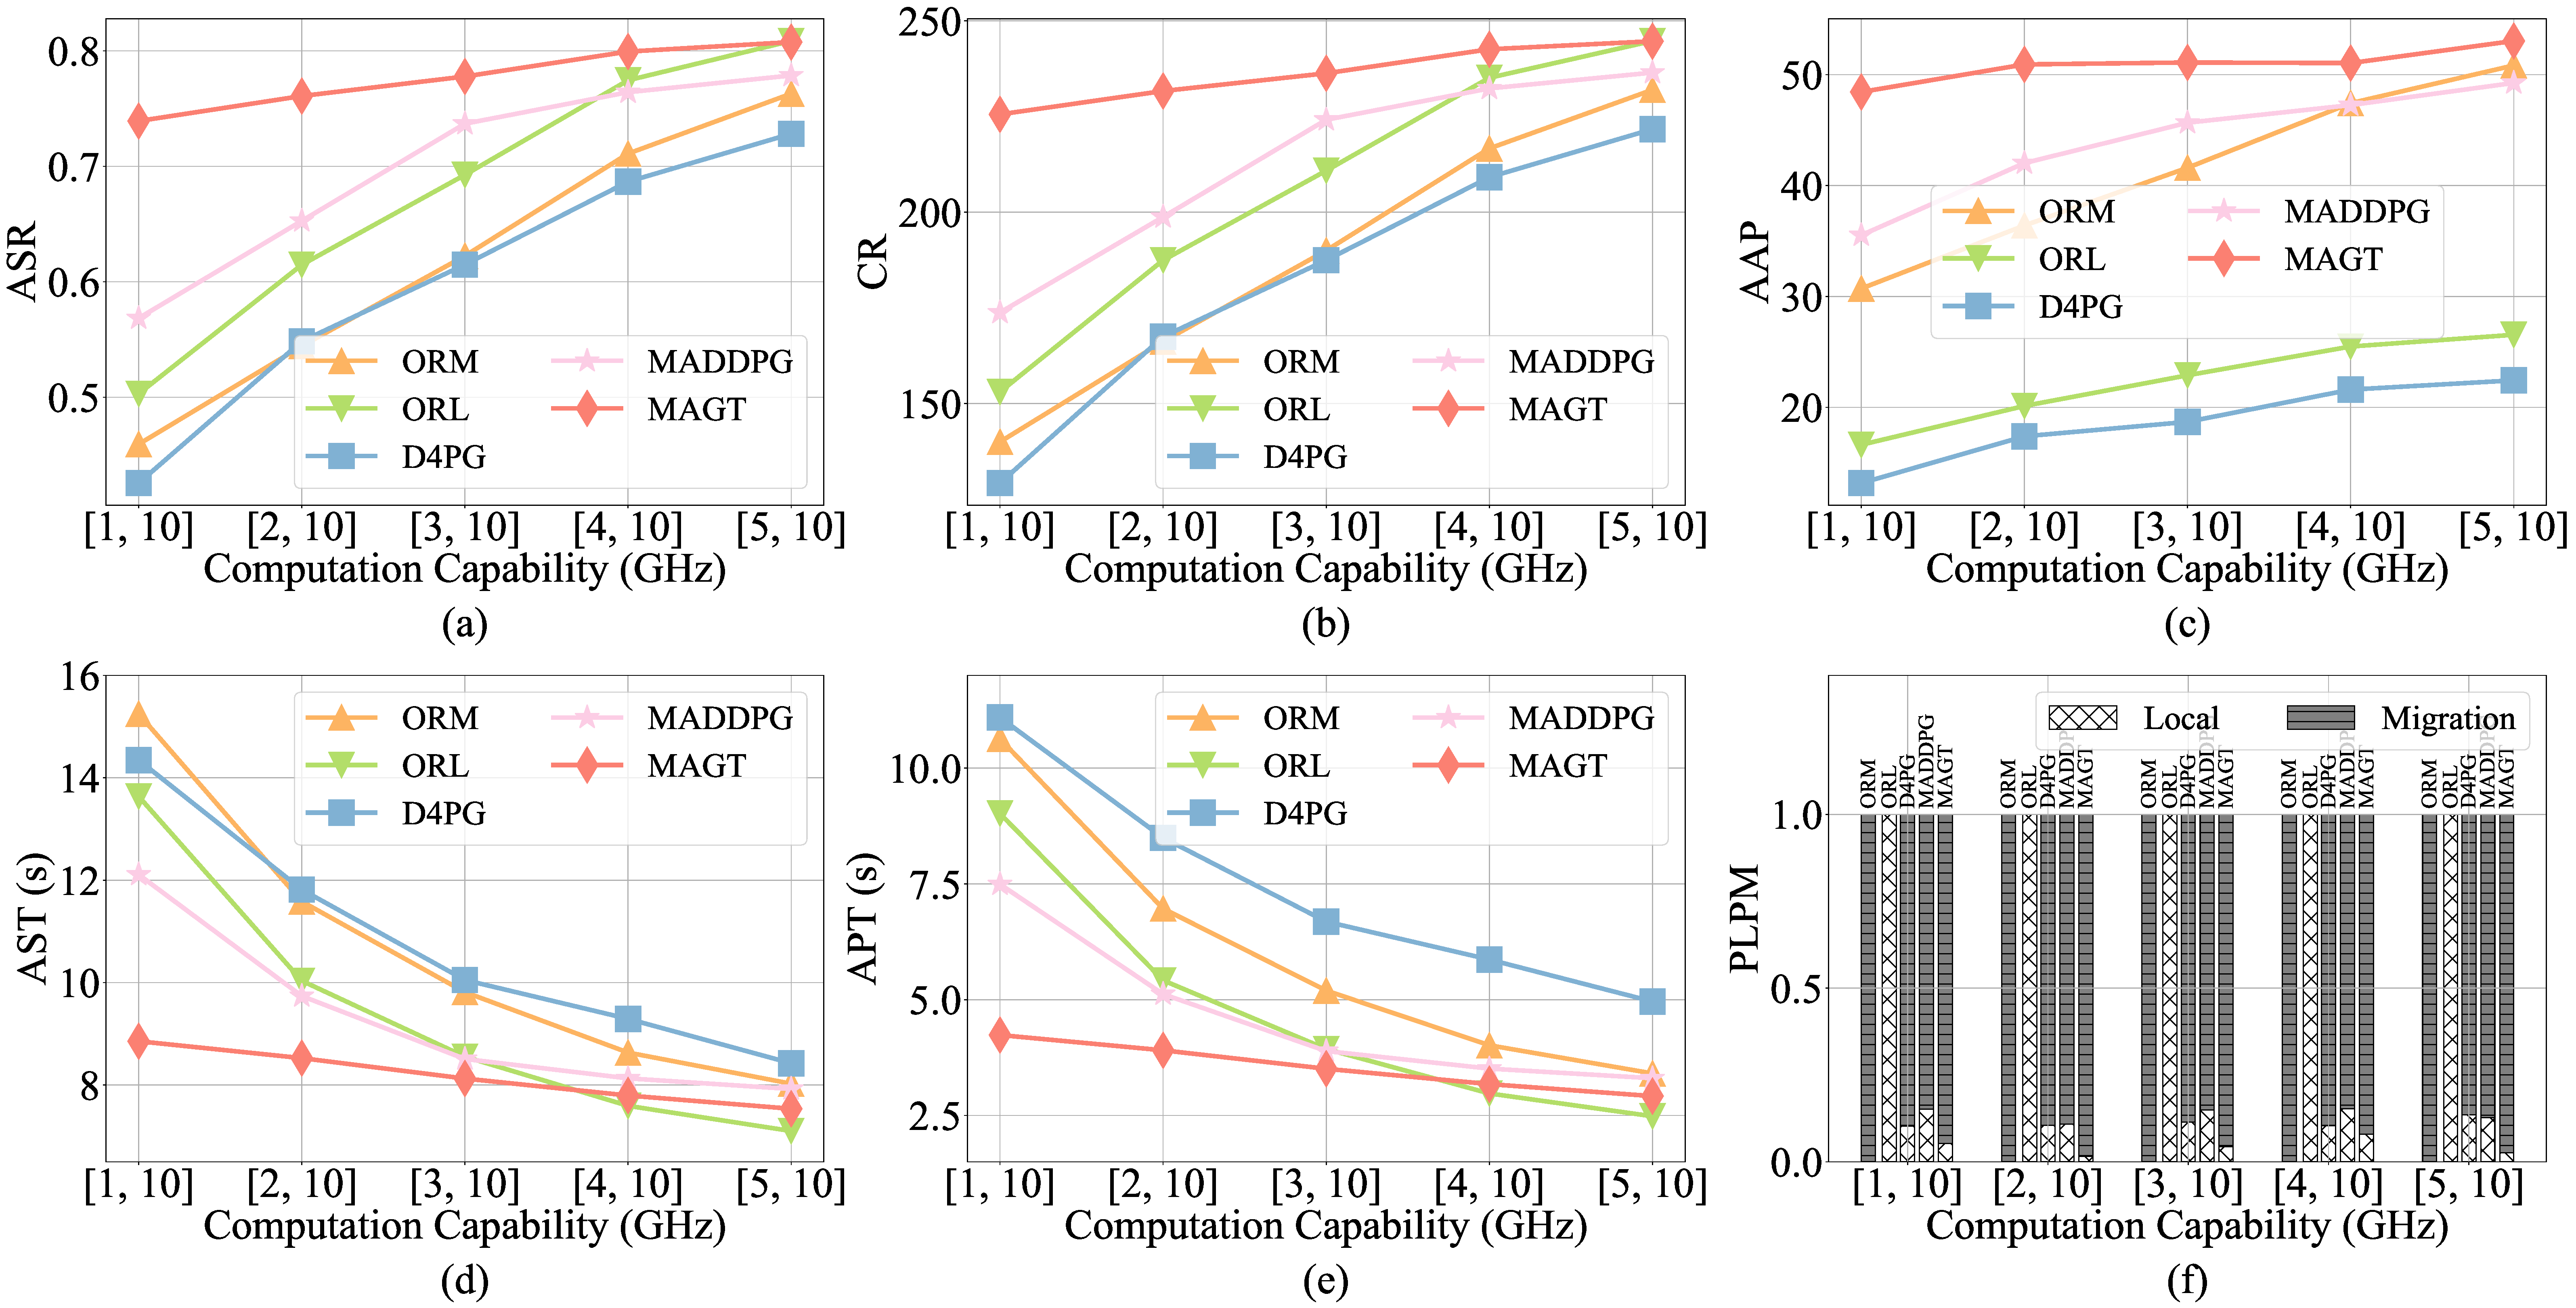
\includegraphics[width=0.9\textwidth]{fig/Fig3-6-different-computation-capability.pdf}
	\end{figure}
\end{textblock*}
\end{center}
}

\only<6-6>{
\begin{center} \englishfont \footnotesize
\begin{textblock*}{\textwidth}(-3.2cm,1.72cm)
{\LARGE{\color{red}\ding{216}}}
\end{textblock*}
\end{center}

\begin{center} \englishfont \footnotesize
\begin{textblock*}{\textwidth}(1cm,1.7cm)
{\LARGE{\color{red}\ding{216}}}
\end{textblock*}
\end{center}

\begin{center} \englishfont \footnotesize
\begin{textblock*}{\textwidth}(5.5cm,1.65cm)
{\LARGE{\color{red}\ding{216}}}
\end{textblock*}
\end{center}

\begin{center} \englishfont \footnotesize
\begin{textblock*}{\textwidth}(0.15cm,6.55cm)
{\LARGE{\color{red}\ding{216}}}
\end{textblock*}
\end{center}

\begin{center} \englishfont \footnotesize
\begin{textblock*}{\textwidth}(-4.2cm,6.5cm)
{\LARGE{\color{red}\ding{216}}}
\end{textblock*}
\end{center}
}

\only<7-7>{
\frametitle{\englishfont \underline{实验}:任务到达概率的影响}
\begin{center} \englishfont \footnotesize
\begin{textblock*}{\textwidth}(1cm,1.8cm)
	\begin{figure}
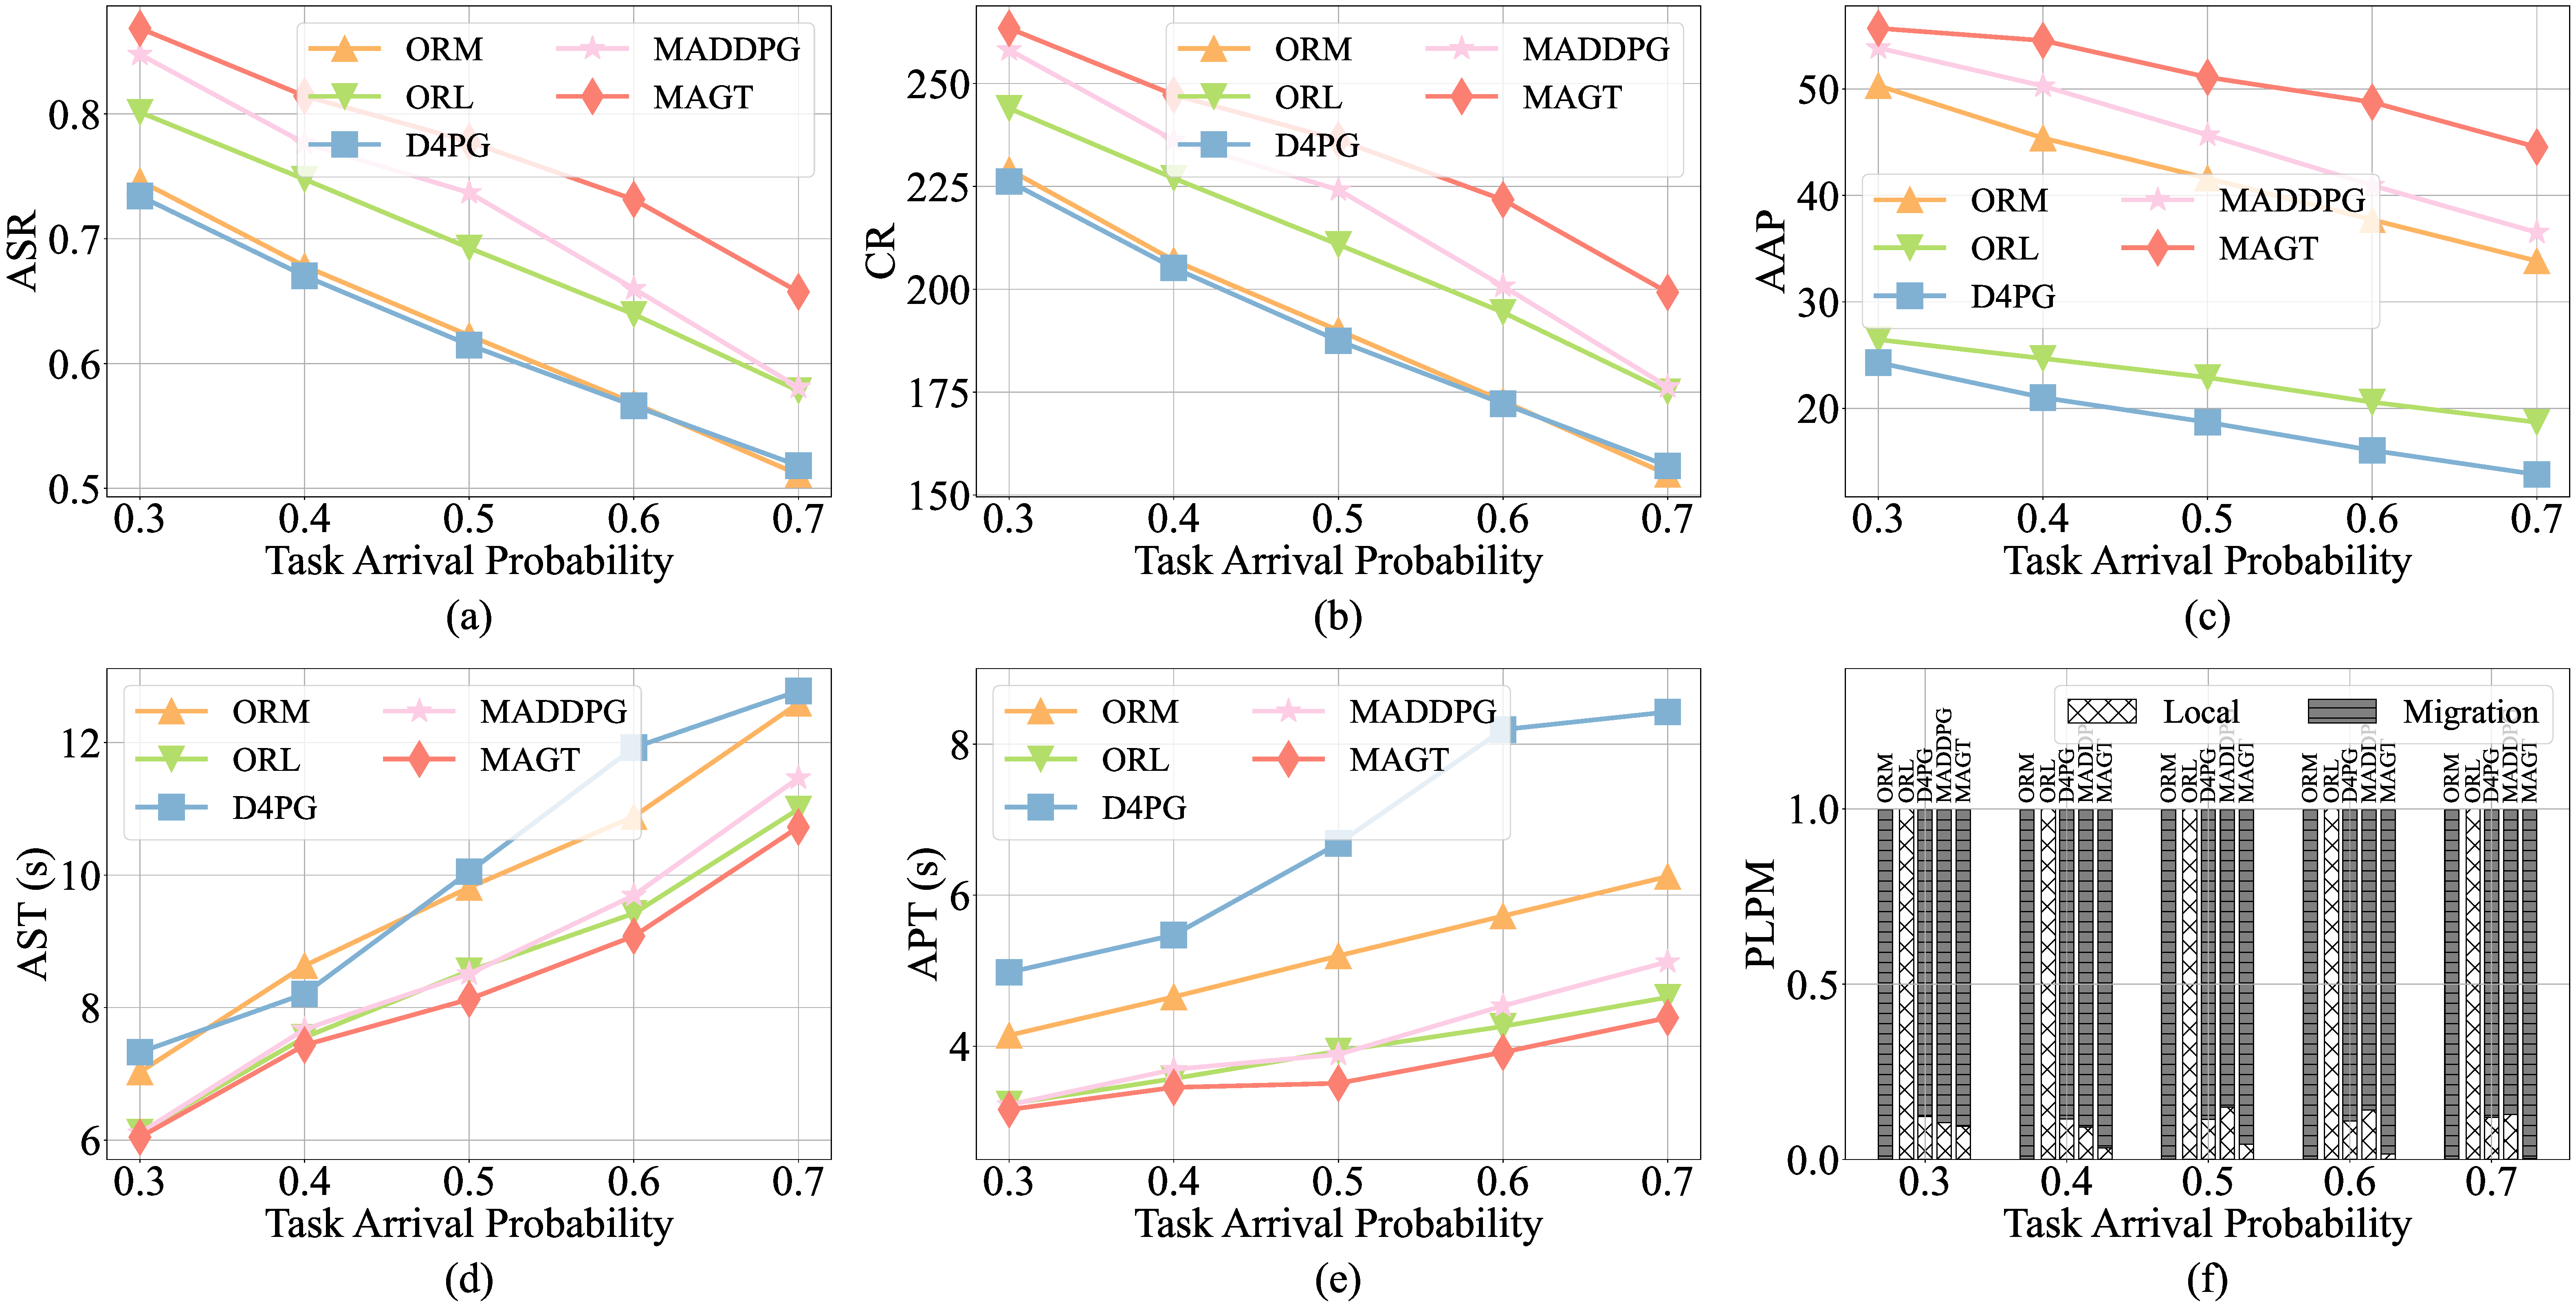
\includegraphics[width=0.9\textwidth]{fig/Fig3-7-different-task-arrival-probability.pdf}
	\end{figure}
\end{textblock*}
\end{center}
}

\only<8-8>{
\frametitle{\englishfont \underline{实验}:任务到达概率的影响}
\begin{center} \englishfont \footnotesize
\begin{textblock*}{\textwidth}(1cm,1.8cm)
	\begin{figure}
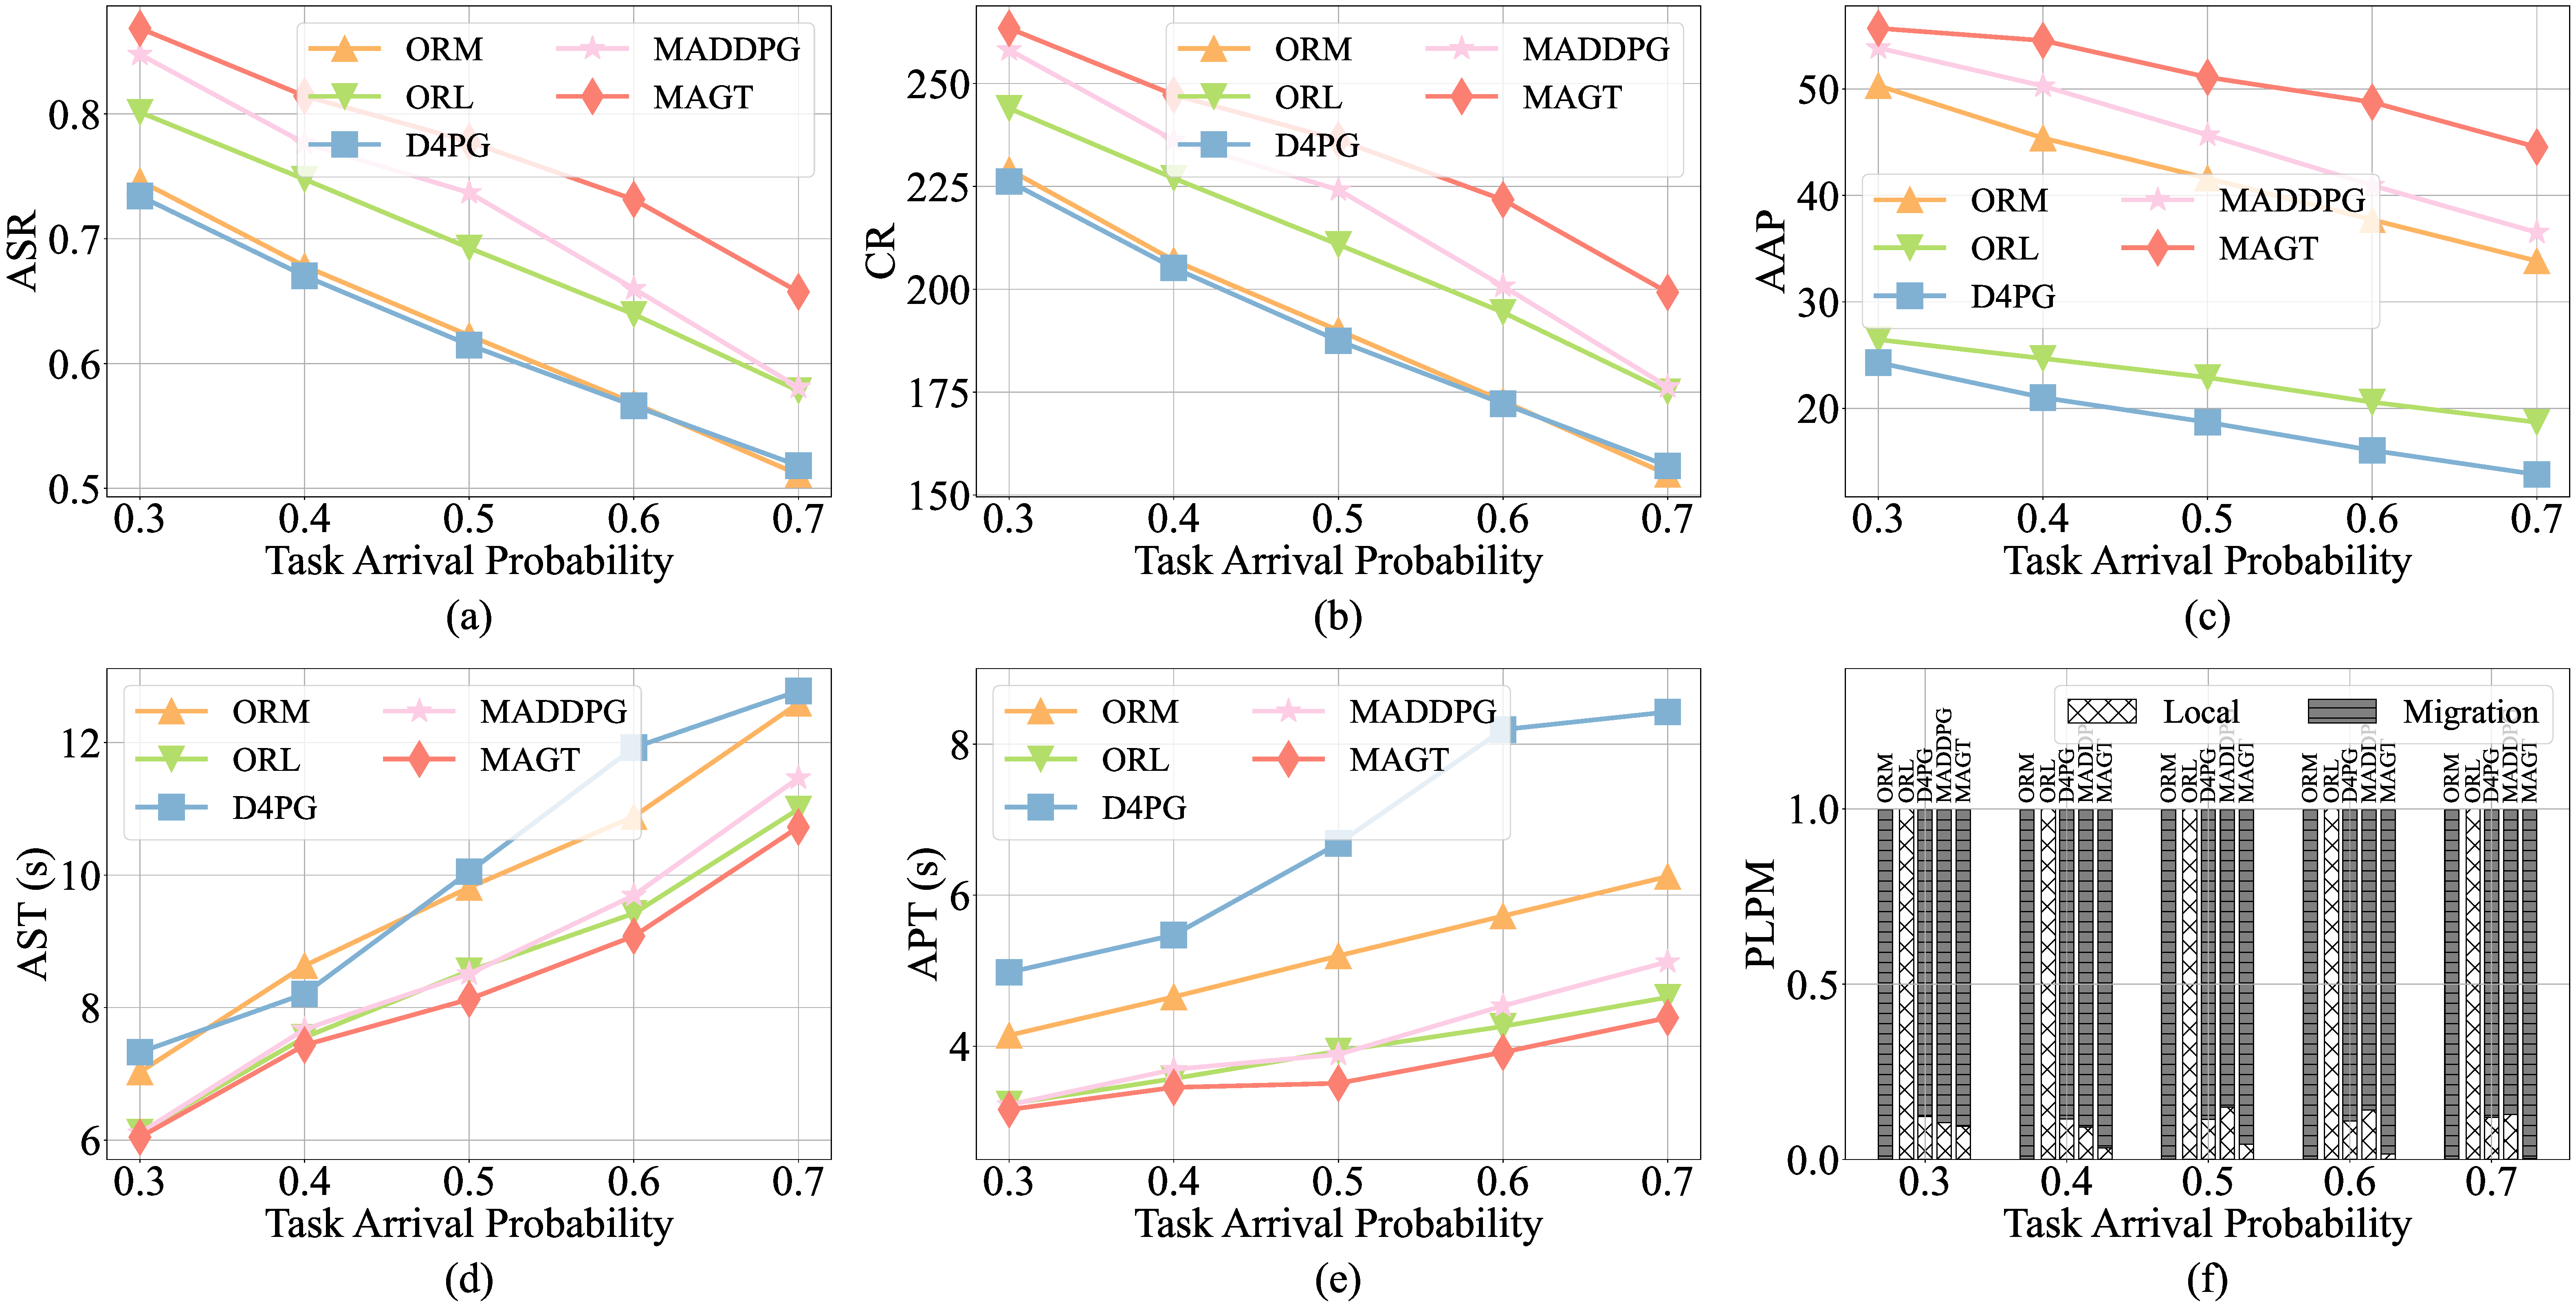
\includegraphics[width=0.9\textwidth]{fig/Fig3-7-different-task-arrival-probability.pdf}
	\end{figure}
\end{textblock*}
\end{center}
}

\only<8-8>{
\begin{center} \englishfont \footnotesize
\begin{textblock*}{\textwidth}(-4.3cm,1.8cm)
{\LARGE{\color{red}\ding{216}}}
\end{textblock*}
\end{center}

\begin{center} \englishfont \footnotesize
\begin{textblock*}{\textwidth}(0cm,1.75cm)
{\LARGE{\color{red}\ding{216}}}
\end{textblock*}
\end{center}

\begin{center} \englishfont \footnotesize
\begin{textblock*}{\textwidth}(5.5cm,1.8cm)
{\LARGE{\color{red}\ding{216}}}
\end{textblock*}
\end{center}

\begin{center} \englishfont \footnotesize
\begin{textblock*}{\textwidth}(0.65cm,6.76cm)
{\LARGE{\color{red}\ding{216}}}
\end{textblock*}
\end{center}

\begin{center} \englishfont \footnotesize
\begin{textblock*}{\textwidth}(-2.7cm,6.2cm)
{\LARGE{\color{red}\ding{216}}}
\end{textblock*}
\end{center}
}
\end{overlayarea}
\end{frame}